% Task C19
% Source volume: lower
% Physical scan pages: 179--199
% Printed book pages: 167--187
% Transcribe only source content; omit running headers, footers, and printed page numbers.
\chapter{偏导数与全微分}

% BEGIN TRANSCRIPTION

本章前两节分别讨论多元函数的偏导数与全微分。在 §19.3 介绍求多元函数偏导数的链式法则。§19.4 是向量值函数的微分学定理。最后一节是学习要点和参考题。方向导数、梯度、Taylor 公式等将在第二十一章（偏导数的应用）中介绍。

\section{偏导数}

\subsection{偏导数的定义}

以二元函数为例。设 $f(x,y)$ 在点 $(x_0,y_0)$ 的某个邻域上有定义。固定 $y=y_0$ 将 $f(x,y)$ 视为 $x$ 的一元函数。如果它在点 $x_0$ 可导，则称此导数是二元函数 $f(x,y)$ 在点 $(x_0,y_0)$ 关于 $x$ 的偏导数，记为 $\frac{\partial f}{\partial x}(x_0,y_0)$ 或 $f_x(x_0,y_0)$，即
\[
  \frac{\partial f}{\partial x}(x_0,y_0)
  =\lim_{\Delta x\to0}\frac{f(x_0+\Delta x,y_0)-f(x_0,y_0)}{\Delta x}.
\]
类似地可以定义 $\frac{\partial f}{\partial y}(x_0,y_0)$ 以及任意个变元的多元函数的偏导数。

\begin{xexample}[19.1.1]
求
\[
  f(x,y)=
  \begin{cases}
    y\ln(x^2+y^2), & (x,y)\ne(0,0),\\
    0, & (x,y)=(0,0)
  \end{cases}
\]
在点 $(0,0)$ 的偏导数。
\end{xexample}
\begin{xsolution}
由于
\[
  \frac{f(\Delta x,0)-f(0,0)}{\Delta x}=\frac{0-0}{\Delta x}=0,
\]
\[
  \frac{f(0,\Delta y)-f(0,0)}{\Delta y}
  =\frac{\Delta y\ln(\Delta y)^2}{\Delta y}=\ln(\Delta y)^2,
\]
从而
\[
  \frac{\partial f}{\partial x}(0,0)=0,
  \qquad
  \frac{\partial f}{\partial y}(0,0)\text{不存在}.
\]
\end{xsolution}

由于多元函数的偏导数是用一元函数的导数来定义的，因此它具有导数的基本性质与运算法则，例如偏导数的四则运算、对复合函数求偏导数的链式法则等。

\paragraph{偏导数的几何意义}
设 $z=f(x,y)$ 是空间 $\RR^3$ 中的曲面，$f(x,y)$ 在点 $(x_0,y_0)$ 的偏导数存在，则它与平面 $y=y_0$ 的交线 $l_x$ 在点 $p_0(x_0,y_0,z_0)$ 处的切向量 $\tau_x$ 为
\[
  \left(1,0,\frac{\partial f}{\partial y}(x_0,y_0)\right),
\]
与平面 $x=x_0$ 的交线 $l_y$ 在点 $p_0(x_0,y_0,z_0)$ 处的切向量 $\tau_y$ 为
\[
  \left(0,1,\frac{\partial f}{\partial x}(x_0,y_0)\right).
\]
% SOURCE-ERR: 原书将 tau_x、tau_y 的第三分量分别印作 \partial f/\partial y 与 \partial f/\partial x；按通常几何意义二者应对调，此处忠实保留原文。

\subsection{偏导数与连续}

在一元函数中，可导可以推出连续。但在多元函数中，若 $f$ 在某一点对每一个变元的偏导数都存在，却不能断言 $f$ 在该点连续，甚至不能断言 $f$ 在该点的极限存在。最简单的例子是
\[
  f(x,y)=
  \begin{cases}
    1, & xy\ne0,\\
    0, & xy=0.
  \end{cases}
\]
显然 $f_x(0,0)=f_y(0,0)=0$，但 $f$ 在点 $(0,0)$ 不连续，甚至极限也不存在。

下面的命题说明，如果偏导数在某一点的邻域上存在而且有界，则可推出函数在该点连续。

\begin{xproposition}[19.1.1]
设函数 $f(x,y)$ 的两个偏导数 $\frac{\partial f}{\partial x}$ 和 $\frac{\partial f}{\partial y}$ 在点 $(x_0,y_0)$ 的某个邻域上存在且有界，则 $f$ 在点 $(x_0,y_0)$ 连续。
\end{xproposition}
\begin{xproof}
注意到
\begin{align*}
  \Delta f
  &=f(x_0+\Delta x,y_0+\Delta y)-f(x_0,y_0)\\
  &=[f(x_0+\Delta x,y_0+\Delta y)-f(x_0,y_0+\Delta y)]
    +[f(x_0,y_0+\Delta y)-f(x_0,y_0)],
\end{align*}
利用一元函数的微分中值定理，得
\[
  \Delta f
  =\frac{\partial f}{\partial x}(x_0+\theta_1\Delta x,y_0+\Delta y)\Delta x
  +\frac{\partial f}{\partial y}(x_0,y_0+\theta_2\Delta y)\Delta y,
\]
其中 $0<\theta_1,\theta_2<1$。已知 $\frac{\partial f}{\partial x},\frac{\partial f}{\partial y}$ 在点 $(x_0,y_0)$ 的邻域上有界，所以
\[
  \lim_{(\Delta x,\Delta y)\to(0,0)}\Delta f=0,
\]
即 $f(x,y)$ 在点 $(x_0,y_0)$ 连续。
\end{xproof}

\subsection{高阶偏导数}

就二元函数而言，若 $f(x,y)$ 的两个偏导数 $f_x(x,y)$ 和 $f_y(x,y)$ 都存在，则它们都是二元函数。如果它们关于 $x$ 的偏导数存在或者关于 $y$ 的偏导数存在，就称这些偏导数是 $f(x,y)$ 的二阶偏导数：
\[
  f\text{ 关于 }x\text{ 的二阶偏导数，记为 }\frac{\partial^2f}{\partial x^2}\text{ 或 }f_{xx};
\]
\[
  f\text{ 关于 }y\text{ 的二阶偏导数，记为 }\frac{\partial^2f}{\partial y^2}\text{ 或 }f_{yy};
\]
\[
  f\text{ 先关于 }x\text{ 后关于 }y\text{ 的二阶混合偏导数，记为 }\frac{\partial^2f}{\partial y\partial x}\text{ 或 }f_{xy};
\]
\[
  f\text{ 先关于 }y\text{ 后关于 }x\text{ 的二阶混合偏导数，记为 }\frac{\partial^2f}{\partial x\partial y}\text{ 或 }f_{yx}.
\]
更高阶的偏导数也可以同样定义。请注意两个混合偏导数 $\frac{\partial^2f}{\partial y\partial x}$ 与 $\frac{\partial^2f}{\partial x\partial y}$ 并不总是相等的，例如设
\[
  f(x,y)=
  \begin{cases}
    xy\dfrac{x^2-y^2}{x^2+y^2}, & (x,y)\ne(0,0),\\
    0, & (x,y)=(0,0).
  \end{cases}
\]
则有
\[
  f_x(x,y)=
  \begin{cases}
    y\dfrac{x^4+4x^2y^2-y^4}{(x^2+y^2)^2}, & (x,y)\ne(0,0),\\
    0, & (x,y)=(0,0),
  \end{cases}
\]
\[
  f_y(x,y)=
  \begin{cases}
    x\dfrac{x^4-4x^2y^2-y^4}{(x^2+y^2)^2}, & (x,y)\ne(0,0),\\
    0, & (x,y)=(0,0).
  \end{cases}
\]
从而在原点处有
\[
  f_{xy}(0,0)=\lim_{\Delta y\to0}\frac{f_x(0,\Delta y)-f_x(0,0)}{\Delta y}=-1,
\]
\[
  f_{yx}(0,0)=\lim_{\Delta x\to0}\frac{f_y(\Delta x,0)-f_y(0,0)}{\Delta x}=1.
\]
由此可见
\[
  f_{yx}(0,0)\ne f_{xy}(0,0).
\]

\begin{xremark}
上面定义的函数 $f(x,y)$ 连续可微（关于可微的定义见下一小节），因为 $f_x$ 和 $f_y$ 都是处处连续的。但如果混合偏导数 $f_{yx}$ 和 $f_{xy}$ 连续，则构造上述反例是不可能的。事实上，如果在某一点 $(x_0,y_0)$ 的邻域内 $f_x,f_y$ 都存在，且 $f_{yx}$ 与 $f_{xy}$ 都在该点连续，那么在点 $(x_0,y_0)$ 一定成立 $f_{yx}=f_{xy}$。在一般的分析教科书上都有这个结论及其证明。我们可以证明下述更强的结论：
\end{xremark}

\begin{xproposition}[19.1.2]
设 $f_x,f_y$ 在点 $(x_0,y_0)$ 的某邻域内存在且 $f_{xy}$ 在点 $(x_0,y_0)$ 连续，则 $f_{yx}(x_0,y_0)$ 存在，且
\[
  f_{yx}(x_0,y_0)=f_{xy}(x_0,y_0).
\]
\end{xproposition}
\begin{xproof}
定义
\[
  \varphi(x)=f(x,y_0+\Delta y)-f(x,y_0).
\]
由于函数 $f$ 存在关于 $x$ 的偏导数，所以 $\varphi(x)$ 可导，应用一元函数的中值定理，有
\begin{align*}
  \varphi(x_0+\Delta x)-\varphi(x_0)
  &=\varphi'(x_0+\theta_1\Delta x)\Delta x\\
  &=[f_x(x_0+\theta_1\Delta x,y_0+\Delta y)-f_x(x_0+\theta_1\Delta x,y_0)]\Delta x,
\end{align*}
其中 $0<\theta_1<1$，又由 $f_x$ 存在关于 $y$ 的偏导数，故对以 $y$ 为自变量的函数 $f_x(x_0+\theta_1\Delta x,y)$ 应用一元函数中值定理，上式化为
\[
  \varphi(x_0+\Delta x)-\varphi(x_0)
  =f_{xy}(x_0+\theta_1\Delta x,y_0+\theta_2\Delta y)\Delta x\Delta y,
\]
其中 $0<\theta_1,\theta_2<1$。因此
\begin{align*}
  &f(x_0+\Delta x,y_0+\Delta y)-f(x_0+\Delta x,y_0)\\
  &\qquad-f(x_0,y_0+\Delta y)+f(x_0,y_0)\\
  &=f_{xy}(x_0+\theta_1\Delta x,y_0+\theta_2\Delta y)\Delta x\Delta y.
\end{align*}
在上式两边同除以 $\Delta y$，并令 $\Delta y\to0$，由偏导数的定义以及 $f_{xy}$ 在点 $(x_0,y_0)$ 连续就得到
\[
  f_y(x_0+\Delta x,y_0)-f_y(x_0,y_0)
  =f_{xy}(x_0+\theta_1\Delta x,y_0)\Delta x.
\]
再在上式两边同除以 $\Delta x$，并令 $\Delta x\to0$，由 $f_{xy}$ 在点 $(x_0,y_0)$ 连续得到
\[
  f_{yx}(x_0,y_0)=f_{xy}(x_0,y_0).
\]
\end{xproof}

\begin{xexample}[19.1.2]
证明：函数
\[
  u(x,t)=\frac{1}{2a\sqrt{\pi t}}\ee^{-\frac{x^2}{4a^2t}}
\]
在上半平面 $\RR^2_+=\{(x,t)\in\RR^2\mid t>0\}$ 上满足热传导方程
\begin{equation}
  \frac{\partial u}{\partial t}-a^2\frac{\partial^2u}{\partial x^2}=0,
  \tag{19.1}
  \label{eq:19.1}
\end{equation}
其中 $a$ 为正常数。
\end{xexample}
\begin{xproof}
$\forall (x,t)\in\RR^2_+$，由于
\begin{align*}
  \frac{\partial u}{\partial t}(x,t)
  &=\frac{1}{2a\sqrt\pi}\left(-\frac{1}{2t^{3/2}}\ee^{-\frac{x^2}{4a^2t}}
    +\frac{1}{t^{1/2}}\ee^{-\frac{x^2}{4a^2t}}\frac{x^2}{4a^2t^2}\right)\\
  &=\frac{1}{4a\sqrt\pi t^{3/2}}\ee^{-\frac{x^2}{4a^2t}}
    \left(-1+\frac{x^2}{2a^2t}\right),
\end{align*}
\[
  \frac{\partial u}{\partial x}(x,t)
  =\frac{1}{2a\sqrt{\pi t}}\ee^{-\frac{x^2}{4a^2t}}
    \left(-\frac{x}{2a^2t}\right),
\]
\begin{align*}
  \frac{\partial^2u}{\partial x^2}(x,t)
  &=\frac{1}{2a\sqrt{\pi t}}
    \left(\ee^{-\frac{x^2}{4a^2t}}\frac{x^2}{4a^4t^2}
      -\frac{1}{2a^2t}\ee^{-\frac{x^2}{4a^2t}}\right)\\
  &=\frac{1}{4a^3\sqrt\pi t^{3/2}}\ee^{-\frac{x^2}{4a^2t}}
    \left(\frac{x^2}{2a^2t}-1\right),
\end{align*}
所以方程 (19.1) 在 $\RR^2_+$ 上成立。
\end{xproof}

\begin{xexample}[19.1.3]
设
\[
  \Gamma(x,y;\xi,\eta)=\frac{1}{2\pi}\ln\sqrt{(x-\xi)^2+(y-\eta)^2},
\]
则
\[
  \left|\frac{\partial\Gamma}{\partial y}\right|
  \le \frac{1}{2\pi}[(x-\xi)^2+(y-\eta)^2]^{-1/2},
\]
\[
  \left|\frac{\partial^2\Gamma}{\partial x\partial y}\right|
  \le \frac{1}{\pi}[(x-\xi)^2+(y-\eta)^2]^{-1}.
\]
\end{xexample}
\begin{xproof}
由于
\[
  \frac{\partial\Gamma}{\partial y}
  =\frac{1}{2\pi}\frac{y-\eta}{(x-\xi)^2+(y-\eta)^2},
\]
\[
  \frac{\partial^2\Gamma}{\partial x\partial y}
  =-\frac{1}{\pi}\frac{(y-\eta)(x-\xi)}{[(x-\xi)^2+(y-\eta)^2]^2},
\]
从而结论成立。
\end{xproof}

\section{全微分}

\subsection{全微分的定义与基本性质}

为方便起见，这里仅讨论二元函数。设 $z=f(x,y)$ 在点 $(x_0,y_0)$ 的某邻域上有定义，如果 $\Delta z=f(x_0+\Delta x,y_0+\Delta y)-f(x_0,y_0)$ 可以表示为
\[
  \Delta z=A\Delta x+B\Delta y+o(r)\quad(r\to0),
\]
其中 $A,B$ 是两个仅与点 $(x_0,y_0)$ 有关而与 $\Delta x,\Delta y$ 无关的常数，$o(r)$ 是当 $r\to0$ 时关于 $r$ 的高阶无穷小量，$r=\sqrt{(\Delta x)^2+(\Delta y)^2}$，则称 $f$ 在点 $(x_0,y_0)$ 可微，且称 $A\Delta x+B\Delta y$ 是函数 $f$ 在点 $(x_0,y_0)$ 的全微分，记作
\[
  \dd z=A\Delta x+B\Delta y.
\]
习惯上，记 $\Delta x=\dd x,\Delta y=\dd y$，于是全微分 $\dd z$ 又可以写为
\[
  \dd z=A\dd x+B\dd y.
\]
从全微分的定义可知，如果函数 $f$ 在点 $(x_0,y_0)$ 可微，那么在点 $(x_0,y_0)$ 附近有
\[
  f(x_0+\Delta x,y_0+\Delta y)\approx f(x_0,y_0)+A\Delta x+B\Delta y.
\]
上式右端是一个线性函数，因此可微的意义在于在点 $(x_0,y_0)$ 附近函数可用关于 $\Delta x$ 与 $\Delta y$ 的一个线性函数近似代替。

全微分具有下列性质：
\begin{enumerate}[label=(\arabic*)]
  \item 如果 $f$ 在点 $(x_0,y_0)$ 可微，则
  \[
    A=\frac{\partial f}{\partial x}(x_0,y_0),\qquad
    B=\frac{\partial f}{\partial y}(x_0,y_0);
  \]
  \item 若 $f$ 在点 $(x_0,y_0)$ 可微，则 $f$ 在点 $(x_0,y_0)$ 连续。
\end{enumerate}
由性质 (1) 知，如果 $f$ 在点 $(x_0,y_0)$ 可微，则 $f$ 在点 $(x_0,y_0)$ 的全微分是
\[
  \dd f=\frac{\partial f}{\partial x}(x_0,y_0)\dd x
  +\frac{\partial f}{\partial y}(x_0,y_0)\dd y.
\]
类似地可定义高阶全微分
\[
  \dd^n f=\dd(\dd^{n-1}f)
  =\left(\dd x\frac{\partial}{\partial x}+\dd y\frac{\partial}{\partial y}\right)^n f,
\]
其中 $\left(\dd x\frac{\partial}{\partial x}+\dd y\frac{\partial}{\partial y}\right)^n$ 是将 $\dd x,\dd y,\frac{\partial}{\partial x},\frac{\partial}{\partial y}$ 视为通常的量按照二项式定理展开而得到的对 $f$ 的一个形式记号，实际上是一个微分算子。

\paragraph{全微分的几何意义}
设 $z=f(x,y)$ 是空间 $\RR^3$ 中的曲面，如果 $f$ 可微，那么在点 $p_0(x_0,y_0,z_0)$ 附近，曲面可以用它在点 $p_0$ 的切平面近似代替。其差是关于
\[
  r=\sqrt{(x-x_0)^2+(y-y_0)^2}
\]
的一个高阶无穷小量，切平面由两个线性无关的切向量 $\tau_x,\tau_y$ 张成，其法向量为
\[
  n=\left(\frac{\partial f}{\partial x}(x_0,y_0),
  \frac{\partial f}{\partial y}(x_0,y_0),-1\right).
\]
与一元函数的情况类似，全微分可用于近似计算与估计误差。以二元函数为例，
\[
  f(x_0+\Delta x,y_0+\Delta y)\approx f(x_0,y_0)
  +\frac{\partial f}{\partial x}(x_0,y_0)\Delta x
  +\frac{\partial f}{\partial y}(x_0,y_0)\Delta y
\]
就是 $(x_0,y_0)$ 附近的一个近似公式；
\[
  \Delta z\approx\frac{\partial f}{\partial x}(x_0,y_0)\Delta x
  +\frac{\partial f}{\partial y}(x_0,y_0)\Delta y
\]
就是点 $(x_0,y_0)$ 附近的一个近似的误差估计式（参见上册 6.3.2 小节中的例题）。

\begin{xexample}[19.2.1]
求 $A=\sqrt{1-(1.004)^2+(1.994)^2}$ 的近似值。
\end{xexample}
\begin{xsolution}
取 $z=f(x,y)=\sqrt{1-x^2+y^2}$，$x_0=1$，$y_0=2$，$\Delta x=0.004$，$\Delta y=-0.006$。计算得
\[
  \frac{\partial f}{\partial x}(1,2)=-\frac12,
  \qquad
  \frac{\partial f}{\partial y}(1,2)=1.
\]
于是
\[
  A=f(1.004,1.994)\approx f(1,2)-\frac12\cdot(0.004)+1\cdot(-0.006)=1.992.
\]
\end{xsolution}

\subsection{多元函数的连续性、偏导数存在性及可微性之间的关系}

多元函数在一个点处的连续性、偏导数存在性及可微性之间有下列关系：
\begin{center}
  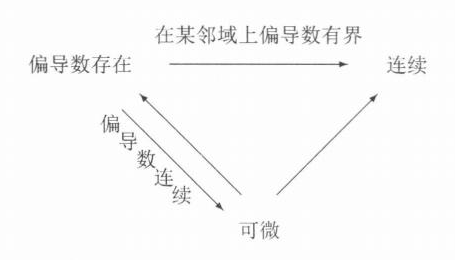
\includegraphics[width=.52\linewidth]{figures/lower/ch19/fig-19-2-relations.png}
\end{center}
由此可得到证明一个函数 $f(x,y)$ 在点 $(x_0,y_0)$ 不可微的常用方法如下：
\begin{enumerate}[label=(\arabic*)]
  \item $f(x,y)$ 在 $(x_0,y_0)$ 点至少有一个偏导数不存在；
  \item $f(x,y)$ 在 $(x_0,y_0)$ 点不连续；
  \item 从定义出发证明 $\Delta f-f_x(x_0,y_0)\Delta x-f_y(x_0,y_0)\Delta y\ne o(r)$。
\end{enumerate}

\begin{xexample}[19.2.2]
设 $f(x,y)=\sqrt{|xy|}$，证明：
\begin{enumerate}[label=(\arabic*)]
  \item $f(x,y)$ 在 $(0,0)$ 点连续；
  \item $\frac{\partial f}{\partial x}(0,0),\frac{\partial f}{\partial y}(0,0)$ 都存在；
  \item $f(x,y)$ 在 $(0,0)$ 点不可微。
\end{enumerate}
\end{xexample}
\begin{xproof}
(1) 由于 $|\Delta f|=|\Delta x|^{1/2}|\Delta y|^{1/2}$，于是
\[
  \lim_{(\Delta x,\Delta y)\to(0,0)}f(x,y)
  =\lim_{(\Delta x,\Delta y)\to(0,0)}[f(0,0)+\Delta f]=0=f(0,0).
\]

(2) 直接按定义计算得
\[
  \frac{\partial f}{\partial x}(0,0)
  =\lim_{\Delta x\to0}\frac{f(\Delta x,0)-f(0,0)}{\Delta x}=0,
\]
\[
  \frac{\partial f}{\partial y}(0,0)
  =\lim_{\Delta y\to0}\frac{f(0,\Delta y)-f(0,0)}{\Delta y}=0.
\]

(3) 由于
\[
  \Delta f-f_x(0,0)\Delta x-f_y(0,0)\Delta y
  =|\Delta x|^{1/2}|\Delta y|^{1/2},
\]
取 $\Delta x=\Delta y\to0$，则
\[
  \frac{\Delta f-f_x(0,0)\Delta x-f_y(0,0)\Delta y}{r}
  =\frac{|\Delta x|^{1/2}|\Delta y|^{1/2}}{\sqrt{(\Delta x)^2+(\Delta y)^2}}
  \to\frac1{\sqrt2}\ne0,
\]
所以 $f(x,y)$ 在 $(0,0)$ 点不可微。
\end{xproof}

\begin{xremark}
$f(x,y)$ 在点 $(x_0,y_0)$ 处可微时，成立无穷小增量公式：
\[
  f(x_0+\Delta x,y_0+\Delta y)
  =f(x_0,y_0)+f_x(x_0,y_0)\Delta x+f_y(x_0,y_0)\Delta y
  +o(|\Delta x|+|\Delta y|).
\]
上述例子说明仅有 $f_x(x_0,y_0),f_y(x_0,y_0)$ 存在还不足以保证二维无穷小增量公式成立。这与一维无穷小增量公式（上册 159 页 (6.1)）成立的条件是不一样的，由此可以体会一元函数与多元函数的区别。
\end{xremark}

\begin{xexample}[19.2.3]
设 $f(x,y)=|x-y|\varphi(x,y)$，其中 $\varphi(x,y)$ 在点 $(0,0)$ 的一个邻域上有定义，要求给函数 $\varphi(x,y)$ 加上适当的条件，使得
\begin{enumerate}[label=(\arabic*)]
  \item $f(x,y)$ 在点 $(0,0)$ 连续；
  \item $f(x,y)$ 在点 $(0,0)$ 存在偏导数；
  \item $f(x,y)$ 在点 $(0,0)$ 可微。
\end{enumerate}
\end{xexample}
\begin{xsolution}
(1) 由于 $f(0,0)=0$，而在点 $(0,0)$ 附近
\[
  |f(x,y)|\le2\sqrt{x^2+y^2}\,|\varphi(x,y)|,
\]
于是当
\[
  \lim_{(x,y)\to(0,0)}\sqrt{x^2+y^2}\,\varphi(x,y)=0
\]
时，$f(x,y)$ 在 $(0,0)$ 点连续。

特别地，当 $\varphi(x,y)$ 在点 $(0,0)$ 附近有界时，$f(x,y)$ 在点 $(0,0)$ 连续。

(2) 由于单侧导数
\begin{align*}
  \left(\frac{\partial f}{\partial x}\right)_{\pm}(0,0)
  &=\lim_{x\to0^{\pm}}\frac{f(x,0)-f(0,0)}{x}\\
  &=\lim_{x\to0^{\pm}}\frac{\pm x\varphi(x,0)}{x}
  =\pm\lim_{x\to0^{\pm}}\varphi(x,0),
\end{align*}
从而当 $\lim_{x\to0^+}\varphi(x,0)=-\lim_{x\to0^-}\varphi(x,0)$ 时，
\[
  \frac{\partial f}{\partial x}(0,0)=\lim_{x\to0^+}\varphi(x,0).
\]
同理当 $\lim_{y\to0^+}\varphi(0,y)=-\lim_{y\to0^-}\varphi(0,y)$ 时，
\[
  \frac{\partial f}{\partial y}(0,0)=\lim_{y\to0^+}\varphi(0,y).
\]
特别地，当 $\lim_{(x,y)\to(0,0)}\varphi(x,y)=0$ 时，
\[
  \frac{\partial f}{\partial x}(0,0)=\frac{\partial f}{\partial y}(0,0)=0.
\]

(3) 由于
\begin{align*}
  &f(x,y)-\frac{\partial f}{\partial x}(0,0)x-\frac{\partial f}{\partial y}(0,0)y\\
  &=|x-y|\varphi(x,y)-\left[\lim_{x\to0^+}\varphi(x,0)\right]x
    -\left[\lim_{y\to0^+}\varphi(0,y)\right]y\\
  &=\begin{cases}
    \left[\varphi(x,y)-\lim_{x\to0^+}\varphi(x,0)\right]x
    -\left[\varphi(x,y)+\lim_{y\to0^+}\varphi(0,y)\right]y, & x\ge y,\\
    -\left[\varphi(x,y)+\lim_{x\to0^+}\varphi(x,0)\right]x
    +\left[\varphi(x,y)-\lim_{y\to0^+}\varphi(0,y)\right]y, & x<y,
  \end{cases}
\end{align*}
由此可以推出，当
\[
  \lim_{(x,y)\to(0,0)}\varphi(x,y)=0
\]
时，$\frac{\partial f}{\partial x}(0,0)=\frac{\partial f}{\partial y}(0,0)=0$ 且 $f(x,y)$ 在 $(0,0)$ 点可微。
\end{xsolution}

\subsection{思考题}

\begin{xthought}[1]
为什么说 $f_x(x_0,y_0)$ 存在就能保证一元函数 $f(x,y_0)$ 在点 $x_0$ 连续？由此能否进一步断言：对充分接近 $y_0$ 的 $y_1$，一元函数 $f(x,y_1)$ 在点 $x_0$ 连续？
\end{xthought}
\begin{xsolution}
$f_x(x_0,y_0)$ 存在，按偏导数定义，就是一元函数
\[
  \varphi(x)=f(x,y_0)
\]
在 $x_0$ 可导。一元函数可导必连续，因此
\[
  \lim_{x\to x_0}f(x,y_0)=f(x_0,y_0).
\]

但不能由此断言当 $y_1$ 充分接近 $y_0$ 时，$x\mapsto f(x,y_1)$ 在 $x_0$ 连续。例如取 $(x_0,y_0)=(0,0)$，定义
\[
  f(x,y)=
  \begin{cases}
    1,&x\ne0,\ y\ne0,\\
    0,&x=0\text{ 或 }y=0.
  \end{cases}
\]
则 $f(x,0)\equiv0$，故 $f_x(0,0)=0$。然而对任意 $y_1\ne0$，都有
\[
  f(0,y_1)=0,\qquad f(x,y_1)=1\quad(x\ne0),
\]
所以 $x\mapsto f(x,y_1)$ 在 $x=0$ 不连续。由于这样的 $y_1$ 可以任意接近 $0$，所述进一步断言不成立。
\end{xsolution}


\begin{xthought}[2]
证明全微分的性质 (1),(2)。
\end{xthought}
\begin{xsolution}
设 $f$ 在 $(x_0,y_0)$ 可微，则
\[
  \Delta f=A\Delta x+B\Delta y+\littleo(r),
  \qquad r=\sqrt{(\Delta x)^2+(\Delta y)^2}.
\]

先证明性质 (1)。令 $\Delta y=0$，则 $r=|\Delta x|$，于是
\[
  \frac{f(x_0+\Delta x,y_0)-f(x_0,y_0)}{\Delta x}
  =A+\frac{\littleo(|\Delta x|)}{\Delta x}.
\]
令 $\Delta x\to0$，右端第二项趋于 $0$，故
\[
  f_x(x_0,y_0)=A.
\]
同理令 $\Delta x=0$，得到
\[
  f_y(x_0,y_0)=B.
\]
因此
\[
  \dd f=f_x(x_0,y_0)\dd x+f_y(x_0,y_0)\dd y.
\]

再证明性质 (2)。由可微公式
\[
  |\Delta f|
  \le |A|\,|\Delta x|+|B|\,|\Delta y|+|\littleo(r)|
  \le (|A|+|B|)r+|\littleo(r)|.
\]
当 $r\to0$ 时右端趋于 $0$，故 $\Delta f\to0$，即 $f$ 在 $(x_0,y_0)$ 连续。
\end{xsolution}


\begin{xthought}[3]
举例说明：
  \begin{enumerate}[label=(\arabic*)]
    \item $f(x,y)$ 在某一点的邻域内存在偏导数，但在该点不一定连续，从而不一定可微；
    \item $f(x,y)$ 在某一点连续，但在该点偏导数不一定存在，从而不一定可微；
    \item $f(x,y)$ 在某一点可微，但在该点偏导数不一定连续。
  \end{enumerate}
\end{xthought}
\begin{xsolution}
分别给出反例。

\textbf{(1)} 定义
\[
  f(x,y)=
  \begin{cases}
    \dfrac{xy}{x^2+y^2},&(x,y)\ne(0,0),\\
    0,&(x,y)=(0,0).
  \end{cases}
\]
在原点以外 $f$ 光滑；而在原点
\[
  f_x(0,0)=\lim_{h\to0}\frac{f(h,0)}h=0,
  \qquad
  f_y(0,0)=\lim_{h\to0}\frac{f(0,h)}h=0.
\]
故两个偏导数在原点的一个邻域内处处存在。但沿 $y=x\ne0$ 有
\[
  f(x,x)=\frac12,
\]
故 $f$ 在原点不连续，从而也不可微。

\textbf{(2)} 取
\[
  f(x,y)=\sqrt{x^2+y^2}.
\]
该函数在原点连续，但
\[
  \frac{f(h,0)-f(0,0)}h=\frac{|h|}{h}
\]
在 $h\to0$ 时无极限，所以 $f_x(0,0)$ 不存在，因而 $f$ 在原点不可微。

\textbf{(3)} 定义
\[
  f(x,y)=
  \begin{cases}
    xy\sin\dfrac1{x^2+y^2},&(x,y)\ne(0,0),\\
    0,&(x,y)=(0,0).
  \end{cases}
\]
在原点 $f_x(0,0)=f_y(0,0)=0$。又令 $r=\sqrt{x^2+y^2}$，则
\[
  \frac{|f(x,y)|}{r}
  \le\frac{|xy|}{r}
  \le\frac{r}{2}\to0,
\]
故 $f$ 在原点可微，且全微分为零。

但当 $(x,y)\ne(0,0)$ 时
\[
  f_x=y\sin\frac1{x^2+y^2}
  -\frac{2x^2y}{(x^2+y^2)^2}\cos\frac1{x^2+y^2}.
\]
沿 $x=y=t$，取 $t_k=(4\pi k)^{-1/2}$，则
\[
  \frac1{2t_k^2}=2\pi k,
\]
从而
\[
  f_x(t_k,t_k)=-\frac1{2t_k}\to-\infty.
\]
所以 $f_x$ 在原点不连续。类似地 $f_y$ 在原点也不连续。这说明可微并不推出偏导数连续。
\end{xsolution}


\begin{xthought}[4]
证明：若 $f_x(x,y)$ 在点 $(x_0,y_0)$ 存在，$f_y(x,y)$ 在点 $(x_0,y_0)$ 连续，则 $f(x,y)$ 在点 $(x_0,y_0)$ 可微。
\end{xthought}
\begin{xsolution}
记 $p=(x_0,y_0)$，并设 $f_x(p)$ 存在、$f_y$ 在 $p$ 连续。将增量分解为
\begin{align*}
  \Delta f
  &=f(x_0+\Delta x,y_0+\Delta y)-f(x_0+\Delta x,y_0)\\
  &\quad+f(x_0+\Delta x,y_0)-f(x_0,y_0).
\end{align*}

由于 $f_y$ 在 $p$ 连续，因而在 $p$ 的某邻域内存在。对第一项把 $x=x_0+\Delta x$ 固定，对变量 $y$ 应用一元函数中值定理，得
\[
  f(x_0+\Delta x,y_0+\Delta y)-f(x_0+\Delta x,y_0)
  =f_y(x_0+\Delta x,y_0+\theta\Delta y)\Delta y,
\]
其中 $0<\theta<1$。由 $f_y$ 在 $p$ 连续，
\[
  f_y(x_0+\Delta x,y_0+\theta\Delta y)
  =f_y(p)+\littleo(1),
\]
故第一项等于
\[
  f_y(p)\Delta y+\littleo(r),
  \qquad r=\sqrt{(\Delta x)^2+(\Delta y)^2}.
\]
另一方面，由 $f_x(p)$ 存在，
\[
  f(x_0+\Delta x,y_0)-f(x_0,y_0)
  =f_x(p)\Delta x+\littleo(|\Delta x|)
  =f_x(p)\Delta x+\littleo(r).
\]
两式相加得到
\[
  \Delta f=f_x(p)\Delta x+f_y(p)\Delta y+\littleo(r),
\]
所以 $f$ 在 $p$ 可微。
\end{xsolution}


\begin{xthought}[5]
设 $z=f(x,y)$ 在开集 $D=(a,b)\times(c,d)$ 上可微，且全微分 $\dd z$ 恒为零。问 $f(x,y)$ 在 $D$ 上是否应取常数值？证明你的结论。
\end{xthought}
\begin{xsolution}
应取常数值。因为 $\dd z\equiv0$，由可微函数全微分的表示式知
\[
  f_x(x,y)=f_y(x,y)=0,
  \qquad (x,y)\in D.
\]
任取 $(x_1,y_1),(x_2,y_2)\in D=(a,b)\times(c,d)$。矩形区域保证线段
\[
  \{(x,y_1):x_1\le x\le x_2\},
  \qquad
  \{(x_2,y):y_1\le y\le y_2\}
\]
均在 $D$ 内。固定 $y=y_1$，一元函数 $x\mapsto f(x,y_1)$ 的导数恒为零，故
\[
  f(x_1,y_1)=f(x_2,y_1).
\]
再固定 $x=x_2$，同理由 $f_y=0$ 得
\[
  f(x_2,y_1)=f(x_2,y_2).
\]
因此
\[
  f(x_1,y_1)=f(x_2,y_2).
\]
两点任意，所以 $f$ 在 $D$ 上为常值函数。
\end{xsolution}


\subsection{练习题}

\begin{xexercise}[1]
设
  \[
    f(x,y)=
    \begin{cases}
      \dfrac{\sqrt{|x-y|}}{x^2+y^2}\sin(x^2+y^2), & x^2+y^2\ne0,\\
      0, & x^2+y^2=0,
    \end{cases}
  \]
  讨论：
  \begin{enumerate}[label=(\arabic*)]
    \item $f(x,y)$ 在点 $(0,0)$ 是否连续？
    \item $f(x,y)$ 在点 $(0,0)$ 是否可微？
  \end{enumerate}
\end{xexercise}
\begin{xsolution}
记 $r=\sqrt{x^2+y^2}$。

\textbf{(1)} 当 $(x,y)\ne(0,0)$ 时，利用 $|\sin r^2|\le r^2$，有
\[
  |f(x,y)|
  =\frac{\sqrt{|x-y|}}{r^2}|\sin r^2|
  \le\sqrt{|x-y|}.
\]
又
\[
  |x-y|\le |x|+|y|\le\sqrt2\,r,
\]
故
\[
  |f(x,y)|\le 2^{1/4}r^{1/2}\to0=f(0,0).
\]
所以 $f$ 在 $(0,0)$ 连续。

\textbf{(2)} 取 $y=0$。当 $h\ne0$ 时
\[
  f(h,0)=\frac{\sqrt{|h|}}{h^2}\sin h^2,
\]
因而
\[
  \frac{f(h,0)-f(0,0)}h
  =\frac{\sqrt{|h|}\sin h^2}{h^3}
  =\frac{\sin h^2}{h^2}\cdot\frac{\sqrt{|h|}}h.
\]
第一因子趋于 $1$，第二因子的绝对值为 $|h|^{-1/2}\to+\infty$，故 $f_x(0,0)$ 不存在。可微必有偏导数，因此 $f$ 在 $(0,0)$ 不可微。
\end{xsolution}


\begin{xexercise}[2]
设
  \[
    f(x,y)=
    \begin{cases}
      xy\sin\dfrac1{x^2+y^2}, & x^2+y^2\ne0,\\
      0, & x^2+y^2=0.
    \end{cases}
  \]
  证明：
  \begin{enumerate}[label=(\arabic*)]
    \item $f_x(0,0),f_y(0,0)$ 都存在；
    \item $f_x(0,0),f_y(0,0)$ 在点 $(0,0)$ 不连续；
    \item $f(x,y)$ 在点 $(0,0)$ 可微。
  \end{enumerate}
  （本题也说明从可微不能推出偏导数连续。）
\end{xexercise}
\begin{xsolution}
\textbf{(1)} 沿坐标轴有 $f(h,0)=f(0,h)=0$，故
\[
  f_x(0,0)=0,
  \qquad
  f_y(0,0)=0.
\]

\textbf{(2)} 当 $(x,y)\ne(0,0)$ 时
\[
  f_x(x,y)=y\sin\frac1{x^2+y^2}
  -\frac{2x^2y}{(x^2+y^2)^2}\cos\frac1{x^2+y^2},
\]
\[
  f_y(x,y)=x\sin\frac1{x^2+y^2}
  -\frac{2xy^2}{(x^2+y^2)^2}\cos\frac1{x^2+y^2}.
\]
令 $x=y=t$，则
\[
  f_x(t,t)=f_y(t,t)
  =t\sin\frac1{2t^2}-\frac1{2t}\cos\frac1{2t^2}.
\]
取 $t_k=(4\pi k)^{-1/2}$，有
\[
  f_x(t_k,t_k)=f_y(t_k,t_k)=-\frac1{2t_k},
\]
其绝对值趋于无穷。因此 $f_x,f_y$ 在 $(0,0)$ 都不连续。

\textbf{(3)} 在原点线性主部为零。由
\[
  |f(x,y)|\le|xy|\le\frac{x^2+y^2}{2}=\frac{r^2}{2}
\]
可得
\[
  \frac{|f(x,y)-f(0,0)-f_x(0,0)x-f_y(0,0)y|}{r}
  \le\frac r2\to0.
\]
故 $f$ 在 $(0,0)$ 可微，且 $\dd f(0,0)=0$。
\end{xsolution}


\begin{xexercise}[3]
设 $f(x,y,z)$ 在开集 $D$ 上有定义，$f_x(x,y,z)$ 与 $f_y(x,y,z)$ 在 $D$ 上有界，且对固定的 $(x,y)$，$f(x,y,z)$ 是 $z$ 的连续函数。证明：$f(x,y,z)$ 在 $D$ 上连续。
\end{xexercise}
\begin{xsolution}
任取 $p=(x_0,y_0,z_0)\in D$。因为 $D$ 为开集，可取 $\rho>0$，使以 $p$ 为中心的一个小长方体完全包含于 $D$。设在 $D$ 上
\[
  |f_x|\le M,
  \qquad
  |f_y|\le M
\]
（若两个界不同，取其较大者）。对充分接近 $p$ 的 $(x,y,z)$，分解
\begin{align*}
  f(x,y,z)-f(x_0,y_0,z_0)
  &=f(x,y,z)-f(x_0,y,z)\\
  &\quad+f(x_0,y,z)-f(x_0,y_0,z)\\
  &\quad+f(x_0,y_0,z)-f(x_0,y_0,z_0).
\end{align*}
前两项分别对 $x,y$ 应用一元函数中值定理，得到
\[
  |f(x,y,z)-f(x_0,y,z)|\le M|x-x_0|,
\]
\[
  |f(x_0,y,z)-f(x_0,y_0,z)|\le M|y-y_0|.
\]
对固定的 $(x_0,y_0)$，题设说明 $z\mapsto f(x_0,y_0,z)$ 在 $z_0$ 连续，因此第三项在 $z\to z_0$ 时趋于 $0$。于是当 $(x,y,z)\to p$ 时三项之和趋于 $0$，故 $f$ 在 $p$ 连续。由于 $p$ 任意，$f$ 在 $D$ 上连续。
\end{xsolution}


\begin{xexercise}[4]
求 $u=\ln(1+x^2+y^2)$ 在 $(x,y)=(1,2)$ 处的全微分。
\end{xexercise}
\begin{xsolution}
设
\[
  u(x,y)=\ln(1+x^2+y^2).
\]
则
\[
  u_x=\frac{2x}{1+x^2+y^2},
  \qquad
  u_y=\frac{2y}{1+x^2+y^2}.
\]
在 $(1,2)$ 处
\[
  u_x(1,2)=\frac13,
  \qquad
  u_y(1,2)=\frac23.
\]
所以
\[
  \boxed{\dd u\big|_{(1,2)}=\frac13\dd x+\frac23\dd y}.
\]
\end{xsolution}


\begin{xexercise}[5]
已测得一圆柱体的底圆直径 $D_0=10.44$，高 $H_0=18.36$，且测量误差 $|\Delta D|\le0.02$，$|\Delta H|\le0.01$。试估计用体积公式 $V=\frac14\pi D^2H$ 计算时的绝对误差 $\Delta V$ 与相对误差 $\Delta V/V$。
\end{xexercise}
\begin{xsolution}
体积
\[
  V(D,H)=\frac\pi4D^2H.
\]
其全微分为
\[
  \dd V=\frac\pi2DH\,\dd D+\frac\pi4D^2\,\dd H.
\]
故绝对误差可用全微分估计为
\begin{align*}
  |\Delta V|
  &\approx |\dd V|\\
  &\le \frac\pi2D_0H_0|\Delta D|
       +\frac\pi4D_0^2|\Delta H|\\
  &\le \frac\pi2(10.44)(18.36)(0.02)
       +\frac\pi4(10.44)^2(0.01)\\
  &=2.189268\pi\approx6.88.
\end{align*}

又
\[
  \frac{\dd V}{V}=2\frac{\dd D}{D}+\frac{\dd H}{H},
\]
所以相对误差满足
\begin{align*}
  \left|\frac{\Delta V}{V}\right|
  &\approx\left|\frac{\dd V}{V}\right|\\
  &\le2\frac{0.02}{10.44}+\frac{0.01}{18.36}\\
  &\approx0.004376,
\end{align*}
即约为
\[
  \boxed{0.438\%}.
\]
相应的绝对误差估计为
\[
  \boxed{|\Delta V|\lesssim6.88}.
\]
\end{xsolution}


\begin{xexercise}[6]
$f(x,y)$ 定义在矩形 $I=[a,b]\times[c,d]$ 上，且 $f_y$ 在 $I$ 上连续，证明：$f(x,y)$ 对 $y$ 满足一致 Lipschitz 条件，即 $\exists L>0$，使得 $\forall(x,y_1),(x,y_2)\in I$，都有
  \[
    |f(x,y_1)-f(x,y_2)|\le L|y_1-y_2|,
  \]
  其中 $L$ 与 $x$ 无关。
\end{xexercise}
\begin{xsolution}
因为 $f_y$ 在紧矩形
\[
  I=[a,b]\times[c,d]
\]
上连续，所以 $f_y$ 在 $I$ 上有界。令
\[
  M=\max_{(x,y)\in I}|f_y(x,y)|<\infty.
\]
固定任意 $x\in[a,b]$，对一元函数 $y\mapsto f(x,y)$ 在 $y_1,y_2$ 之间应用中值定理，存在介于 $y_1,y_2$ 之间的 $\xi$，使
\[
  f(x,y_1)-f(x,y_2)=f_y(x,\xi)(y_1-y_2).
\]
于是
\[
  |f(x,y_1)-f(x,y_2)|
  \le M|y_1-y_2|.
\]
若 $M>0$，取 $L=M$；若 $M=0$，可任取 $L>0$。这个 $L$ 与 $x$ 无关，故 $f$ 对 $y$ 满足一致 Lipschitz 条件。
\end{xsolution}


\begin{xexercise}[7]
若函数 $f(x,y)$ 的偏导数 $f_x$ 和 $f_y$ 在区域 $D$ 内存在，且 $\forall(x,y)\in D$，$f_x(x,y)=f_y(x,y)=0$。证明：$f(x,y)$ 在 $D$ 上为常值函数。
\end{xexercise}
\begin{xsolution}
任取 $p\in D$。因为 $D$ 是区域，特别是开集，所以存在以 $p$ 为中心的小矩形 $R\subset D$。在 $R$ 内任取两点 $(x_1,y_1),(x_2,y_2)$。先固定 $y=y_1$，由 $f_x=0$ 和一元函数中值定理，
\[
  f(x_1,y_1)=f(x_2,y_1).
\]
再固定 $x=x_2$，由 $f_y=0$，
\[
  f(x_2,y_1)=f(x_2,y_2).
\]
所以 $f$ 在每个这样的 $R$ 上为常数，即 $f$ 在 $D$ 上局部常值。

局部常值函数在每个连通分支上为常数，而“区域”按定义是连通开集。因此 $f$ 在整个 $D$ 上为常值函数。
\end{xsolution}


\begin{xexercise}[8]
设 $\Omega\in\RR^2$ 是开区域，$u(x,y),v(x,y)$ 在 $\Omega$ 内满足
  \[
    \frac{\partial u}{\partial x}=\frac{\partial v}{\partial y},
    \qquad
    \frac{\partial u}{\partial y}=-\frac{\partial v}{\partial x},
    \qquad
    u^2+v^2=C,
  \]
  其中 $C$ 为常数，证明：$u(x,y),v(x,y)$ 在 $\Omega$ 上均为常值函数。
\end{xexercise}
\begin{xsolution}
由
\[
  u^2+v^2=C
\]
分别对 $x,y$ 求偏导，得
\[
  u u_x+v v_x=0,
  \qquad
  u u_y+v v_y=0.
\]
再利用
\[
  u_x=v_y,
  \qquad
  u_y=-v_x,
\]
可改写为
\[
  u u_x-v u_y=0,
  \qquad
  v u_x+u u_y=0.
\]
即
\[
  \begin{pmatrix}
    u&-v\\
    v&u
  \end{pmatrix}
  \binom{u_x}{u_y}=0.
\]
其系数行列式为
\[
  u^2+v^2=C.
\]
若 $C=0$，则 $u=v=0$，结论显然。若 $C>0$，系数矩阵可逆，从而
\[
  u_x=u_y=0.
\]
再由 Cauchy--Riemann 型关系得到
\[
  v_x=-u_y=0,
  \qquad
  v_y=u_x=0.
\]
由上一题的结论，$u,v$ 在区域 $\Omega$ 上都为常值函数。
\end{xsolution}


\begin{xexercise}[9]
设 $f(x,y)$ 在 $G=\{(x,y)\mid x^2+y^2<1\}$ 上有定义。若 $f(x,0)$ 在点 $x=0$ 处连续，且 $f_y(x,y)$ 在 $G$ 上有界。证明：$f(x,y)$ 在点 $(0,0)$ 处连续。
\end{xexercise}
\begin{xsolution}
设
\[
  |f_y(x,y)|\le M,
  \qquad (x,y)\in G.
\]
当 $(x,y)$ 充分接近 $(0,0)$ 时，竖直线段从 $(x,0)$ 到 $(x,y)$ 完全包含在圆盘 $G$ 中。对 $y$ 应用一元函数中值定理，得
\[
  |f(x,y)-f(x,0)|\le M|y|.
\]
于是
\[
  |f(x,y)-f(0,0)|
  \le M|y|+|f(x,0)-f(0,0)|.
\]
当 $(x,y)\to(0,0)$ 时，第一项趋于 $0$；第二项由题设 $f(x,0)$ 在 $x=0$ 连续也趋于 $0$。因此
\[
  \lim_{(x,y)\to(0,0)}f(x,y)=f(0,0),
\]
即 $f$ 在 $(0,0)$ 连续。
\end{xsolution}


\section{复合函数求导（链式法则）}

\subsection{复合函数偏导数的链式法则}

若 $z=f(u_1,u_2,\cdots,u_m)$ 在点 $(u_1,u_2,\cdots,u_m)$ 可微，$u_i=g_i(x_1,x_2,\cdots,x_n)$ $(i=1,2,\cdots,m)$ 在点 $(x_1,x_2,\cdots,x_n)$ 有关于 $x_j$ $(j=1,2,\cdots,n)$ 的偏导数，则复合函数
\[
  z=f[g_1(x_1,x_2,\cdots,x_n),g_2(x_1,x_2,\cdots,x_n),\cdots,g_m(x_1,x_2,\cdots,x_n)]
\]
关于自变量 $x_j$ 的偏导数存在且
\begin{equation}
  \frac{\partial z}{\partial x_j}
  =\sum_{i=1}^m\frac{\partial f}{\partial u_i}\cdot\frac{\partial u_i}{\partial x_j},
  \qquad j=1,2,\cdots,n.
  \tag{19.2}
  \label{eq:19.2}
\end{equation}
写成矩阵的形式为
\[
  \left(\frac{\partial z}{\partial x_1},\frac{\partial z}{\partial x_2},\cdots,\frac{\partial z}{\partial x_n}\right)
  =\left(\frac{\partial f}{\partial u_1},\frac{\partial f}{\partial u_2},\cdots,\frac{\partial f}{\partial u_m}\right)
  \begin{pmatrix}
    \frac{\partial u_1}{\partial x_1} & \frac{\partial u_1}{\partial x_2} & \cdots & \frac{\partial u_1}{\partial x_n}\\
    \frac{\partial u_2}{\partial x_1} & \frac{\partial u_2}{\partial x_2} & \cdots & \frac{\partial u_2}{\partial x_n}\\
    \vdots & \vdots & & \vdots\\
    \frac{\partial u_m}{\partial x_1} & \frac{\partial u_m}{\partial x_2} & \cdots & \frac{\partial u_m}{\partial x_n}
  \end{pmatrix}.
\]

\paragraph{特款 1}
若 $z=f(x,y)$，而 $x=\varphi(t)$，$y=\psi(t)$，则
\begin{equation}
  \frac{\dd z}{\dd t}=\frac{\partial f}{\partial x}\varphi'(t)+\frac{\partial f}{\partial y}\psi'(t).
  \tag{19.3}
  \label{eq:19.3}
\end{equation}

\paragraph{特款 2}
若 $z=f(x,y,t)$，而 $x=\varphi(s,t)$，$y=\psi(s,t)$，则
\begin{equation}
  \frac{\partial z}{\partial s}
  =\frac{\partial f}{\partial x}\frac{\partial\varphi}{\partial s}
  +\frac{\partial f}{\partial y}\frac{\partial\psi}{\partial s},
  \tag{19.4}
  \label{eq:19.4}
\end{equation}
\begin{equation}
  \frac{\partial z}{\partial t}
  =\frac{\partial f}{\partial x}\frac{\partial\varphi}{\partial t}
  +\frac{\partial f}{\partial y}\frac{\partial\psi}{\partial t}
  +\frac{\partial f}{\partial t}.
  \tag{19.5}
  \label{eq:19.5}
\end{equation}
注意：最后一个等式左边的 $\frac{\partial z}{\partial t}$ 与等式右边的 $\frac{\partial f}{\partial t}$ 不一样，$\frac{\partial z}{\partial t}$ 表示函数
\[
  z=f[\varphi(s,t),\psi(s,t),t]
\]
对 $t$ 求偏导，此时视 $s$ 为常数，而 $\frac{\partial f}{\partial t}$ 是 $z=f(x,y,t)$ 对 $t$ 求偏导，把 $x,y$ 视为常数。为了避免混乱，有时引入下面的记号
\[
  f_1=\frac{\partial f}{\partial x}(x,y,t),\qquad
  f_2=\frac{\partial f}{\partial y}(x,y,t),\qquad
  f_3=\frac{\partial f}{\partial t}(x,y,t),
\]
其中下标 $i$ $(i=1,2,3)$ 表示对第 $i$ 个自变量求偏导，于是可将 (19.4),(19.5) 写为
\[
  z_s=f_1\varphi_s+f_2\psi_s,\qquad
  z_t=f_1\varphi_t+f_2\psi_t+f_3.
\]
写成矩阵的形式为
\[
  (z_s,z_t)=(f_1,f_2,f_3)
  \begin{pmatrix}
    \varphi_s & \varphi_t\\
    \psi_s & \psi_t\\
    0 & 1
  \end{pmatrix}.
\]

\subsection{例题}

\begin{xexample}[19.3.1]
对于幂指函数 $u=x^y$，令 $x=\varphi(t),y=\psi(t)$，求 $\frac{\dd u}{\dd t}$。
\end{xexample}
\begin{xsolution}
由 (19.3) 得
\begin{align*}
  \frac{\dd u}{\dd t}
  &=\frac{\partial u}{\partial x}\varphi'(t)+\frac{\partial u}{\partial y}\psi'(t)\\
  &=yx^{y-1}\varphi'(t)+x^y\ln x\,\psi'(t)
   =x^y\left(\frac{y}{x}\varphi'(t)+\ln x\,\psi'(t)\right)\\
  &=[\varphi(t)]^{\psi(t)}\left\{\frac{\psi(t)}{\varphi(t)}\varphi'(t)+[\ln\varphi(t)]\psi'(t)\right\}.
\end{align*}
（以前我们曾用另外的方法证明过它，参见上册 165--166 页的对数求导法。）
\end{xsolution}

作为公式 (19.3) 的另一个应用，讨论行列式
\[
  \Delta=
  \begin{vmatrix}
    a_{11}&a_{12}&\cdots&a_{1n}\\
    a_{21}&a_{22}&\cdots&a_{2n}\\
    \vdots&\vdots&&\vdots\\
    a_{n1}&a_{n2}&\cdots&a_{nn}
  \end{vmatrix}
\]
的求导，其中假定元素 $a_{ij}$ $(i,j=1,2,\cdots,n)$ 都是 $t$ 的一元函数，它们关于 $t$ 的导数 $\frac{\dd a_{ij}}{\dd t}$ 都存在。

\begin{xexample}[19.3.2]
证明：行列式 $\Delta$ 的导数等于把 $\Delta$ 内的第 1 行直到第 $n$ 行的元素依次换成它们的导数而得出的 $n$ 个行列式之和。
\end{xexample}
\begin{xproof}
回忆行列式关于第 $i$ 行元素的展开式
\[
  \Delta=\sum_{j=1}^n A_{ij}a_{ij},
\]
其中 $A_{ij}$ 为 $a_{ij}$ 的代数余子式。容易看出 $A_{i1},A_{i2},\cdots,A_{in}$ 中不含有元素 $a_{ij}$，$1\le j\le n$，于是
\[
  \frac{\partial\Delta}{\partial a_{ij}}=A_{ij}.
\]
按照公式 (19.3) 有
\[
  \frac{\dd\Delta}{\dd t}
  =\sum_{i=1}^n\sum_{j=1}^n\frac{\partial\Delta}{\partial a_{ij}}\cdot\frac{\dd a_{ij}}{\dd t}
  =\sum_{i=1}^n\sum_{j=1}^n A_{ij}\frac{\dd a_{ij}}{\dd t}.
\]
注意到 $\sum_{j=1}^n A_{ij}\frac{\dd a_{ij}}{\dd t}$ 也表示一个行列式的展开式，它同已知行列式 $\Delta$ 的差别仅在于把 $\Delta$ 中第 $i$ 行的元素 $a_{i1},a_{i2},\cdots,a_{in}$ 换成它们的导数 $\frac{\dd a_{i1}}{\dd t},\frac{\dd a_{i2}}{\dd t},\cdots,\frac{\dd a_{in}}{\dd t}$，由此可知结论成立。
\end{xproof}

\begin{xremark}
在使用链式法则 (19.2) 时，要求 $f(u_1,u_2,\cdots,u_m)$ 在点 $(u_1,u_2,\cdots,u_m)$ 可微，否则公式 (19.2) 有可能失效，请看下面的例子：
\[
  f(x,y)=
  \begin{cases}
    \dfrac{x^2y}{x^2+y^2}, & (x,y)\ne(0,0),\\
    0, & (x,y)=(0,0).
  \end{cases}
\]
由于
\[
  f_x(x,y)=
  \begin{cases}
    \dfrac{2xy^3}{(x^2+y^2)^2}, & (x,y)\ne(0,0),\\
    0, & (x,y)=(0,0),
  \end{cases}
\]
\[
  f_y(x,y)=
  \begin{cases}
    \dfrac{x^2(x^2-y^2)}{(x^2+y^2)^2}, & (x,y)\ne(0,0),\\
    0, & (x,y)=(0,0),
  \end{cases}
\]
可以看出 $f_x$ 与 $f_y$ 都在 $(0,0)$ 点不连续，容易证明 $f(x,y)$ 在 $(0,0)$ 点不可微。令 $x=y=t$，则 $f(t,t)=\frac12t$，从而 $\frac{\dd f}{\dd t}=\frac12$。如果用链式法则，有
\[
  \frac{\dd f}{\dd t}=f_xx'+f_yy'.
\]
当 $(x,y)=(0,0)$ 时，$\frac{\dd f}{\dd t}=0$。问题出在 $f(x,y)$ 在点 $(0,0)$ 不可微，也就是不满足链式法则的条件。
\end{xremark}

\begin{xexample}[19.3.3]
设 $f(x,y)$ 在 $\RR^2$ 上有连续偏导数，且 $f(x,x^2)=1$。
\begin{enumerate}[label=(\arabic*)]
  \item 若 $f_x(x,x^2)=x$，求 $f_y(x,x^2)$；
  \item 若 $f_y(x,y)=x^2+2y$，求 $f(x,y)$。
\end{enumerate}
\end{xexample}
\begin{xsolution}
(1) 对 $f(x,x^2)=1$ 两边求导得
\[
  f_x+2xf_y=0.
\]
由条件得
\[
  x+2xf_y=0,
\]
所以当 $x\ne0$ 时，$f_y(x,x^2)=-\frac12$。由 $f_y$ 的连续性知，当 $x=0$ 时也有 $f_y(x,x^2)=-\frac12$。

(2) 令 $F(x,y)=f(x,y)-(x^2y+y^2)$，则 $F(x,y)$ 在 $\RR^2$ 上连续可微，且
\[
  F_y(x,y)=0.
\]
于是 $F(x,y)$ 只是 $x$ 的函数，即 $F(x,y)=\varphi(x)$，从而
\[
  f(x,y)=x^2y+y^2+\varphi(x).
\]
再由 $f(x,x^2)=1$ 得 $\varphi(x)=1-2x^4$，所以
\[
  f(x,y)=x^2y+y^2+1-2x^4.
\]
\end{xsolution}

\begin{xexample}[19.3.4]
设 $u=f(x,y)$，$v=g(x,y,u)$，$w=h(x,u,v)$，求 $\frac{\partial w}{\partial x},\frac{\partial w}{\partial y}$。
\end{xexample}
\begin{xsolution}
复合这几个函数得到
\[
  w=h[x,f(x,y),g(x,y,f(x,y))].
\]
从而
\[
  \frac{\partial w}{\partial x}
  =h_1+h_2\frac{\partial f}{\partial x}+h_3\left(g_1+g_3\frac{\partial f}{\partial x}\right),
\]
\[
  \frac{\partial w}{\partial y}
  =h_2\frac{\partial f}{\partial y}+h_3\left(g_2+g_3\frac{\partial f}{\partial y}\right).
\]
\end{xsolution}

\begin{xexample}[19.3.5]
设二元连续可微函数 $F$ 在直角坐标下可写为 $F(x,y)=f(x)g(y)$，在极坐标中可写为 $F(r\cos\theta,r\sin\theta)=h(r)$。若 $F(x,y)$ 无零点，求 $F(x,y)$。
\end{xexample}
\begin{xsolution}
注意
\begin{align*}
  \frac{\partial F}{\partial\theta}
  &=\frac{\partial F}{\partial x}\frac{\partial x}{\partial\theta}
    +\frac{\partial F}{\partial y}\frac{\partial y}{\partial\theta}\\
  &=f'(x)g(y)(-r\sin\theta)+f(x)g'(y)r\cos\theta\\
  &=-yf'(x)g(y)+xf(x)g'(y).
\end{align*}
另一方面有
\[
  \frac{\partial F}{\partial\theta}=\frac{\partial h(r)}{\partial\theta}=0.
\]
于是 $-yf'(x)g(y)+xf(x)g'(y)=0$。当 $x\ne0,y\ne0$ 时有
\begin{equation}
  \frac{f'(x)}{xf(x)}=\frac{g'(y)}{yg(y)}.
  \tag{19.6}
  \label{eq:19.6}
\end{equation}
由于上式对任意的 $x\ne0,y\ne0$ 恒成立，于是
\begin{equation}
  \frac{f'(x)}{xf(x)}=\frac{g'(y)}{yg(y)}=\lambda,
  \tag{19.7}
  \label{eq:19.7}
\end{equation}
其中 $\lambda$ 为任一常数。由 (19.7) 得
\[
  \frac{f'(x)}{f(x)}=\lambda x,
\]
即 $(\ln f)'=\left(\frac\lambda2x^2\right)'$，所以
\begin{equation}
  \ln f(x)=\frac\lambda2x^2+C,
  \tag{19.8}
  \label{eq:19.8}
\end{equation}
其中 $C$ 为任意常数。由 (19.8) 得到
\[
  f(x)=C_1\ee^{\lambda x^2/2},
\]
其中 $C_1$ 为任意常数。由 (19.7) 还可得到
\[
  g(y)=C_2\ee^{\lambda y^2/2},
\]
其中 $C_2$ 为任意常数。最后得到
\[
  F(x,y)=C\ee^{\lambda(x^2+y^2)/2},
\]
其中 $C,\lambda$ 为任意常数。$F(x,y)$ 在 $x=0$ 或 $y=0$ 的值由连续性得到。
\end{xsolution}

\begin{xexample}[19.3.6]
设 $a,b\ne0$，$f$ 具有二阶连续偏导数，且
\begin{equation}
  a^2\frac{\partial^2f}{\partial x^2}+b^2\frac{\partial^2f}{\partial y^2}=0,
  \tag{19.9}
\end{equation}
\begin{equation}
  f(ax,bx)=ax,
  \tag{19.10}
\end{equation}
\begin{equation}
  f_x(ax,bx)=bx^2.
  \tag{19.11}
\end{equation}
求 $f_{xx}(ax,bx),f_{xy}(ax,bx),f_{yy}(ax,bx)$。
\end{xexample}
\begin{xsolution}
对 (19.10) 两边求导，得
\begin{equation}
  af_x(ax,bx)+bf_y(ax,bx)=a.
  \tag{19.12}
\end{equation}
对 (19.11),(19.12) 两边求导得
\begin{equation}
  af_{xx}(ax,bx)+bf_{xy}(ax,bx)=2bx,
  \tag{19.13}
\end{equation}
\begin{equation}
  a^2f_{xx}(ax,bx)+2abf_{xy}(ax,bx)+b^2f_{yy}(ax,bx)=0.
  \tag{19.14}
\end{equation}
由 (19.9),(19.14) 得
\begin{equation}
  f_{xy}(ax,bx)=0.
  \tag{19.15}
\end{equation}
将 (19.15) 代入 (19.13) 得
\begin{equation}
  f_{xx}(ax,bx)=\frac{2b}{a}x.
  \tag{19.16}
\end{equation}
最后将 (19.16) 代入 (19.9) 得
\[
  f_{yy}(ax,bx)=-\frac{2a}{b}x.
\]
\end{xsolution}

\subsection{齐次函数}

\begin{xdefinition}
如果函数 $f(x,y)$ 满足 $f(tx,ty)=t^n f(x,y)$，其中 $t>0$，则称 $f$ 是 $n$ 次齐次函数。
\end{xdefinition}
齐次函数有如下性质：

\begin{xproposition}[19.3.1]
设 $f$ 有连续偏导数，则 $f$ 是 $n$ 次齐次函数的充分必要条件是
\[
  x\frac{\partial f}{\partial x}(x,y)+y\frac{\partial f}{\partial y}(x,y)=nf(x,y).
\]
\end{xproposition}

\begin{xproposition}[19.3.2]
设 $f(x,y)$ 是二次连续可微的 $n$ 次齐次函数，则
\[
  \left(x\frac{\partial}{\partial x}+y\frac{\partial}{\partial y}\right)^2f(x,y)=n(n-1)f(x,y),
\]
这里
\[
  \left(x\frac{\partial}{\partial x}+y\frac{\partial}{\partial y}\right)^2
  =x^2\left(\frac{\partial}{\partial x}\right)^2
  +2xy\left(\frac{\partial}{\partial x}\right)\left(\frac{\partial}{\partial y}\right)
  +y^2\left(\frac{\partial}{\partial y}\right)^2
\]
是一种缩写的形式记号，即把 $x,y,\frac{\partial}{\partial x},\frac{\partial}{\partial y}$ 都看成为常数后按二项式展开，但并不是将算子 $x\frac{\partial}{\partial x}+y\frac{\partial}{\partial y}$ 对 $f(x,y)$ 接连作用两次。
\end{xproposition}

\begin{xproposition}[19.3.3]
若 $f(x,y)$ 是二次连续可微的 $n$ 次齐次函数，则 $f_x(x,y),f_y(x,y)$ 是 $(n-1)$ 次齐次函数。
\end{xproposition}

\begin{xproposition}[19.3.4]
若 $f(x,y)$ 是在 $\RR^2\setminus\{0\}$ 上连续的 $n$ 次齐次函数，则
\[
  |f(x,y)|\le C(x^2+y^2)^{n/2},
\]
其中 $C$ 为正常数。
\end{xproposition}

以上命题都可以推广到任意个自变量的情形。它们的证明都不难，留给读者。

\begin{xexample}[19.3.7]
证明：
\[
  u=\varphi\left(\frac yx\right)+y\psi\left(\frac yx\right)
\]
满足方程
\begin{equation}
  x^2\frac{\partial^2u}{\partial x^2}+2xy\frac{\partial^2u}{\partial x\partial y}+y^2\frac{\partial^2u}{\partial y^2}=0,
  \tag{19.17}
\end{equation}
其中 $\varphi,\psi$ 均为二次连续可微函数。
\end{xexample}
\begin{xsolution}
当然可以通过复合函数求导数来验证方程，但观其特点，首先是由 $\varphi$ 和 $\psi$ 的任意性知 $\varphi(y/x)$ 与 $y\psi(y/x)$ 都应该满足方程。又注意到 $\varphi(y/x)$ 为零次齐次函数，$y\psi(y/x)$ 为一次齐次函数，且方程 (19.17) 可写为
\[
  \left(x\frac{\partial}{\partial x}+y\frac{\partial}{\partial y}\right)^2u=0.
\]
由命题 19.3.2 知
\[
  \left(x\frac{\partial}{\partial x}+y\frac{\partial}{\partial y}\right)^2\varphi\left(\frac yx\right)
  =0(0-1)\varphi\left(\frac yx\right)=0,
\]
\[
  \left(x\frac{\partial}{\partial x}+y\frac{\partial}{\partial y}\right)^2\left[y\psi\left(\frac yx\right)\right]
  =1\cdot0\cdot\left[y\psi\left(\frac yx\right)\right]=0.
\]
于是
\[
  \left(x\frac{\partial}{\partial x}+y\frac{\partial}{\partial y}\right)^2
  \left[\varphi\left(\frac yx\right)+y\psi\left(\frac yx\right)\right]=0.
\]
这就是所要证明的。
\end{xsolution}

\subsection{练习题}

\begin{xexercise}[1]
设 $u=\ee^x+\sin y+t$，$x=st$，$y=s+t$，求 $\frac{\partial u}{\partial t}$。
\end{xexercise}
\begin{xsolution}
由链式法则
\[
  \frac{\partial u}{\partial t}
  =\ee^x\frac{\partial x}{\partial t}
   +\cos y\frac{\partial y}{\partial t}+1.
\]
因为 $x=st,y=s+t$，故
\[
  \frac{\partial x}{\partial t}=s,
  \qquad
  \frac{\partial y}{\partial t}=1.
\]
因此
\[
  \boxed{\frac{\partial u}{\partial t}
  =s\ee^{st}+\cos(s+t)+1}.
\]
\end{xsolution}


\begin{xexercise}[2]
设 $u=f(s,t)$，$s=\frac{x}{y}$，$t=\frac{y}{z}$，求 $\frac{\partial u}{\partial x},\frac{\partial u}{\partial y},\frac{\partial u}{\partial z}$。
\end{xexercise}
\begin{xsolution}
由于 $s=x/y$、$t=y/z$，以下计算在 $y\ne0$、$z\ne0$ 的定义域内进行。记 $f_s=\frac{\partial f}{\partial s}$，$f_t=\frac{\partial f}{\partial t}$，它们均在
\[
  s=\frac xy,
  \qquad
  t=\frac yz
\]
处取值。由链式法则
\[
  \boxed{\frac{\partial u}{\partial x}=\frac1y f_s},
\]
\[
  \boxed{\frac{\partial u}{\partial y}
  =-\frac{x}{y^2}f_s+\frac1z f_t},
\]
\[
  \boxed{\frac{\partial u}{\partial z}
  =-\frac{y}{z^2}f_t}.
\]
\end{xsolution}


\begin{xexercise}[3]
设 $u=f(s,t,y)$，$s=\varphi(x,y)$，$t=\psi(x,y)$，求 $\frac{\partial u}{\partial x},\frac{\partial u}{\partial y}$。
\end{xexercise}
\begin{xsolution}
把 $f$ 的三个自变量依次记为 $(s,t,y)$。由链式法则
\[
  \boxed{
  \frac{\partial u}{\partial x}
  =f_s\varphi_x+f_t\psi_x},
\]
而对 $y$ 求偏导时，第三个自变量 $y$ 本身还贡献一项，因此
\[
  \boxed{
  \frac{\partial u}{\partial y}
  =f_s\varphi_y+f_t\psi_y+f_y}.
\]
其中 $f_s,f_t,f_y$ 均在
\[
  (s,t,y)=(\varphi(x,y),\psi(x,y),y)
\]
处取值。
\end{xsolution}


\begin{xexercise}[4]
设 $u=\ee^x\sin y$，$x=2st$，$y=t+s^2$，求 $\frac{\partial u}{\partial s},\frac{\partial u}{\partial t}$。
\end{xexercise}
\begin{xsolution}
由
\[
  u=\ee^{2st}\sin(t+s^2)
\]
直接求偏导，得
\[
  \boxed{
  \frac{\partial u}{\partial s}
  =\ee^{2st}\left[2t\sin(t+s^2)+2s\cos(t+s^2)\right]},
\]
\[
  \boxed{
  \frac{\partial u}{\partial t}
  =\ee^{2st}\left[2s\sin(t+s^2)+\cos(t+s^2)\right]}.
\]
\end{xsolution}


\begin{xexercise}[5]
设 $u=f(ax^2+by^2+cz^2)$，求 $\dd u$。
\end{xexercise}
\begin{xsolution}
令
\[
  q=ax^2+by^2+cz^2.
\]
则 $u=f(q)$，故
\[
  \dd u=f'(q)\dd q
  =f'(q)(2ax\dd x+2by\dd y+2cz\dd z).
\]
即
\[
  \boxed{\dd u
  =2f'(ax^2+by^2+cz^2)
  (ax\dd x+by\dd y+cz\dd z)}.
\]
\end{xsolution}


\begin{xexercise}[6]
设 $f(x,y,z)=\left(\frac xy\right)^{1/z}$，求 $\dd f(1,1,1)$。
\end{xexercise}
\begin{xsolution}
在 $(1,1,1)$ 的邻域内可写
\[
  f(x,y,z)=\exp\left[\frac1z(\ln x-\ln y)\right].
\]
因此
\[
  f_x=\frac{f}{zx},
  \qquad
  f_y=-\frac{f}{zy},
  \qquad
  f_z=-\frac{f}{z^2}(\ln x-\ln y).
\]
在 $(1,1,1)$ 处，$f=1$，于是
\[
  f_x=1,
  \qquad f_y=-1,
  \qquad f_z=0.
\]
所以
\[
  \boxed{\dd f(1,1,1)=\dd x-\dd y}.
\]
\end{xsolution}


\begin{xexercise}[7]
设 $w=F(xy,yz)$，$F$ 为有连续偏导数的二元函数，证明：
  \[
    x\frac{\partial w}{\partial x}+z\frac{\partial w}{\partial z}=y\frac{\partial w}{\partial y}.
  \]
\end{xexercise}
\begin{xsolution}
令
\[
  p=xy,
  \qquad q=yz,
  \qquad w=F(p,q).
\]
则
\[
  w_x=F_p y,
  \qquad
  w_z=F_q y,
  \qquad
  w_y=F_p x+F_q z.
\]
从而
\[
  xw_x+zw_z
  =xyF_p+zyF_q
  =y(xF_p+zF_q)
  =yw_y.
\]
故
\[
  \boxed{x\frac{\partial w}{\partial x}
  +z\frac{\partial w}{\partial z}
  =y\frac{\partial w}{\partial y}}.
\]
\end{xsolution}


\begin{xexercise}[8]
设 $z=f(xy)$，$f$ 为可微的一元函数，证明：
  \[
    x\frac{\partial z}{\partial x}-y\frac{\partial z}{\partial y}=0.
  \]
\end{xexercise}
\begin{xsolution}
设 $s=xy$。由链式法则
\[
  z_x=f'(s)y,
  \qquad
  z_y=f'(s)x.
\]
故
\[
  xz_x-yz_y
  =xyf'(s)-xyf'(s)=0.
\]
即
\[
  \boxed{x\frac{\partial z}{\partial x}
  -y\frac{\partial z}{\partial y}=0}.
\]
\end{xsolution}


\begin{xexercise}[9]
设二元函数 $u=F(x,y)$ 满足方程
  \[
    x\frac{\partial u}{\partial x}+y\frac{\partial u}{\partial y}=0,
  \]
  证明：$F(x,y)$ 在极坐标系下只是 $\theta$ 的函数。
\end{xexercise}
\begin{xsolution}
令
\[
  U(r,\theta)=F(r\cos\theta,r\sin\theta).
\]
当 $r>0$ 时，由链式法则
\begin{align*}
  \frac{\partial U}{\partial r}
  &=F_x\cos\theta+F_y\sin\theta\\
  &=\frac1r(xF_x+yF_y)=0.
\end{align*}
因此对每个固定的 $\theta$，$U(r,\theta)$ 与 $r$ 无关，故存在一元函数 $h$，使
\[
  \boxed{F(r\cos\theta,r\sin\theta)=h(\theta)}
\]
（在 $r>0$ 的定义域内）。也就是说，$F$ 在极坐标下只是 $\theta$ 的函数。
\end{xsolution}


\begin{xexercise}[10]
设二元函数 $F$ 在直角坐标系中可写成 $F(x,y)=f(x)g(y)$，在极坐标中可写成 $F(r\cos\theta,r\sin\theta)=h(\theta)$，求 $F(x,y)$。
\end{xexercise}
\begin{xsolution}
在 $F=f(x)g(y)$ 非零的连通部分上，由题设 $F(r\cos\theta,r\sin\theta)=h(\theta)$ 可知 $F$ 与 $r$ 无关。因此
\[
  0=\frac{\partial F}{\partial r}
  =F_x\cos\theta+F_y\sin\theta.
\]
乘以 $r$，得到
\[
  xf'(x)g(y)+yf(x)g'(y)=0.
\]
在 $x,y,f(x),g(y)$ 均非零处除以 $f(x)g(y)$，有
\[
  x\frac{f'(x)}{f(x)}
  =-y\frac{g'(y)}{g(y)}.
\]
左端只依赖 $x$，右端只依赖 $y$，故二者必为同一常数 $\lambda$：
\[
  x\frac{f'(x)}{f(x)}=\lambda,
  \qquad
  y\frac{g'(y)}{g(y)}=-\lambda.
\]
于是
\[
  f(x)=C_1|x|^\lambda,
  \qquad
  g(y)=C_2|y|^{-\lambda}
\]
（在固定符号的区间内）。故在每个不穿过坐标轴的连通分支上
\[
  \boxed{F(x,y)=C\left|\frac{x}{y}\right|^\lambda}.
\]
若限定在 $x>0,y>0$，则可写成
\[
  \boxed{F(x,y)=C\left(\frac{x}{y}\right)^\lambda}.
\]
恒零函数也是题设的解。若还要求跨坐标轴或在原点连续可微，则应再按相应定义域的正则性要求对上述常数和指数作限制。
\end{xsolution}


\begin{xexercise}[11]
证明：$u=\varphi(x+at)+\psi(x-at)$ 满足方程
  \[
    \frac{\partial^2u}{\partial t^2}-a^2\frac{\partial^2u}{\partial x^2}=0,
  \]
  其中 $\varphi,\psi$ 为具有二阶连续导数的一元函数。
\end{xexercise}
\begin{xsolution}
令
\[
  \xi=x+at,
  \qquad
  \eta=x-at,
  \qquad
  u=\varphi(\xi)+\psi(\eta).
\]
则
\[
  u_x=\varphi'(\xi)+\psi'(\eta),
  \qquad
  u_t=a\varphi'(\xi)-a\psi'(\eta).
\]
再求一次偏导：
\[
  u_{xx}=\varphi''(\xi)+\psi''(\eta),
\]
\[
  u_{tt}=a^2\varphi''(\xi)+a^2\psi''(\eta).
\]
所以
\[
  \boxed{u_{tt}-a^2u_{xx}=0}.
\]
\end{xsolution}


\begin{xexercise}[12]
设 $x=x(u,v),y=y(u,v)$ 满足
  \[
    \frac{\partial x}{\partial u}=\frac{\partial y}{\partial v},
    \qquad
    \frac{\partial x}{\partial v}=-\frac{\partial y}{\partial u},
  \]
  又设 $w=w(x,y)$ 满足方程
  \[
    \frac{\partial^2w}{\partial x^2}+\frac{\partial^2w}{\partial y^2}=0,
  \]
  证明：
  \begin{enumerate}[label=(\arabic*)]
    \item $w=w(x(u,v),y(u,v))$ 满足方程 $\frac{\partial^2w}{\partial u^2}+\frac{\partial^2w}{\partial v^2}=0$；
    \item $\frac{\partial^2(xy)}{\partial u^2}+\frac{\partial^2(xy)}{\partial v^2}=0$。
  \end{enumerate}
\end{xexercise}
\begin{xsolution}
为书写简洁，记复合函数仍为
\[
  w(u,v)=w(x(u,v),y(u,v)).
\]
题设关系为
\[
  x_u=y_v,
  \qquad
  x_v=-y_u.
\]
题目涉及关于 $u,v$ 的二阶偏导，因此以下按这些复合函数所需的二阶偏导存在且混合偏导可交换来计算。于是由题设关系进一步有
\[
  x_{uu}+x_{vv}=y_{vu}-y_{uv}=0,
\]
\[
  y_{uu}+y_{vv}=-x_{vu}+x_{uv}=0.
\]
此外
\[
  x_u y_u+x_v y_v
  =y_vy_u-y_uy_v=0,
\]
以及
\[
  x_u^2+x_v^2=y_u^2+y_v^2.
\]

\textbf{(1)} 由二阶链式法则
\begin{align*}
  w_{uu}+w_{vv}
  &=(x_u^2+x_v^2)w_{xx}
    +2(x_uy_u+x_vy_v)w_{xy}\\
  &\quad +(y_u^2+y_v^2)w_{yy}
    +(x_{uu}+x_{vv})w_x
    +(y_{uu}+y_{vv})w_y\\
  &=(x_u^2+x_v^2)(w_{xx}+w_{yy})=0.
\end{align*}
故
\[
  \boxed{w_{uu}+w_{vv}=0}.
\]

\textbf{(2)} 把上一结论应用于 $w(x,y)=xy$。因为
\[
  w_{xx}=w_{yy}=0,
\]
所以 $w=xy$ 是关于 $(x,y)$ 的调和函数。故复合后
\[
  \boxed{
  \frac{\partial^2(xy)}{\partial u^2}
  +\frac{\partial^2(xy)}{\partial v^2}=0}.
\]
\end{xsolution}


\begin{xexercise}[13]
证明：可微函数 $z=f(x,y)$ 仅是 $ax+by$ $(ab\ne0)$ 的函数的充分必要条件是
  \[
    b\frac{\partial z}{\partial x}=a\frac{\partial z}{\partial y}.
  \]
\end{xexercise}
\begin{xsolution}
先证必要性。若
\[
  z=f(x,y)=\varphi(ax+by),
\]
则
\[
  z_x=a\varphi'(ax+by),
  \qquad
  z_y=b\varphi'(ax+by),
\]
所以
\[
  bz_x=az_y.
\]

再证充分性。设
\[
  bz_x=az_y.
\]
作可逆线性变换
\[
  s=ax+by,
  \qquad
  t=bx-ay.
\]
其逆变换为
\[
  x=\frac{as+bt}{a^2+b^2},
  \qquad
  y=\frac{bs-at}{a^2+b^2}.
\]
令
\[
  Z(s,t)=z(x(s,t),y(s,t)).
\]
则
\begin{align*}
  Z_t
  &=z_x\frac{b}{a^2+b^2}
    +z_y\frac{-a}{a^2+b^2}\\
  &=\frac{bz_x-az_y}{a^2+b^2}=0.
\end{align*}
因此 $Z$ 与 $t$ 无关，存在一元函数 $\varphi$ 使
\[
  Z(s,t)=\varphi(s).
\]
还原变量得到
\[
  \boxed{z=f(x,y)=\varphi(ax+by)}.
\]
故所给条件充分且必要。
\end{xsolution}


\begin{xexercise}[14]
设 $u(x,y)$ 有连续二阶偏导数，$F(s,t)$ 有连续一阶偏导数，且满足
  \[
    F(u_x,u_y)=0,\qquad F_s^2+F_t^2\ne0,
  \]
  证明：$u_{xx}u_{yy}-u_{xy}^2=0$。
\end{xexercise}
\begin{xsolution}
由
\[
  F(u_x,u_y)=0
\]
分别对 $x,y$ 求偏导，得到
\[
  F_su_{xx}+F_tu_{xy}=0,
\]
\[
  F_su_{xy}+F_tu_{yy}=0.
\]
即
\[
  \begin{pmatrix}
    u_{xx}&u_{xy}\\
    u_{xy}&u_{yy}
  \end{pmatrix}
  \binom{F_s}{F_t}=0.
\]
题设
\[
  F_s^2+F_t^2\ne0
\]
说明向量 $(F_s,F_t)^T$ 非零。于是上面的 $2\times2$ 矩阵有非零核向量，故其行列式为零：
\[
  \boxed{u_{xx}u_{yy}-u_{xy}^2=0}.
\]
\end{xsolution}


\begin{xexercise}[15]
设 $u=f(\sqrt{x^2+y^2})$ 有连续二阶偏导数，且满足 $\frac{\partial^2u}{\partial x^2}+\frac{\partial^2u}{\partial y^2}=0$。试求 $u(x,y)$。
\end{xexercise}
\begin{xsolution}
令
\[
  r=\sqrt{x^2+y^2},
  \qquad u(x,y)=f(r).
\]
当 $r>0$ 时
\[
  u_x=f'(r)\frac xr,
  \qquad
  u_y=f'(r)\frac yr.
\]
计算得
\[
  u_{xx}+u_{yy}=f''(r)+\frac1r f'(r).
\]
故调和方程等价于
\[
  f''(r)+\frac1r f'(r)=0,
\]
即
\[
  (r f'(r))'=0.
\]
因此
\[
  r f'(r)=C_1,
  \qquad
  f(r)=C_1\ln r+C_2.
\]
所以在不含原点的区域上，径向解为
\[
  \boxed{u(x,y)=C_1\ln\sqrt{x^2+y^2}+C_2}.
\]
若题设的“有连续二阶偏导数”是指 $u$ 在包含原点的整个邻域内为 $C^2$ 函数，则 $\ln r$ 在 $r=0$ 无法连续延拓，必须有 $C_1=0$。此时
\[
  \boxed{u(x,y)=C_2},
\]
即只有常值解。
\end{xsolution}


\section{向量值函数的微分学定理}

\subsection{无穷小增量公式与拟微分平均值定理}

设 $D$ 是 $\RR^n$ 中的一个开集，$f\colon D\to\RR^m$ 是一个向量值函数，即
\[
  f(x)=(f_1(x),f_2(x),\cdots,f_m(x)),\qquad x=(x_1,x_2,\cdots,x_n),
\]
其中 $f_1,f_2,\cdots,f_m$ 均是 $n$ 元实函数。当 $f_1,f_2,\cdots,f_m$ 均是 $D$ 上的可微函数时，称 $f$ 是 $D$ 上的可微向量值函数，或者是 $D$ 上的可微映射。当 $f$ 在点 $x_0\in D$ 处可微时，称 Jacobi（雅可比）矩阵
\[
  \left(\frac{\partial f_i}{\partial x_j}(x_0)\right)_{m\times n}
\]
为 $f$ 在点 $x_0$ 处的全导数，记为 $f'(x_0)$（又记为 $Jf(x_0)$），它表示了一个自 $\RR^n$ 到 $\RR^m$ 的线性变换。当 $f$ 在点 $x_0$ 处可微时，我们有如下无穷小增量公式，它给出了向量值函数的差的局部估计。

\begin{xproposition}[19.4.1]
设开区域 $D\subset\RR^n$，$f\colon D\to\RR^m$ 在 $D$ 上可微，点 $x_0,x\in D$，则
\[
  f(x)=f(x_0)+Jf(x_0)(x-x_0)+o(x-x_0),
\]
其中 $o(x-x_0)$ 表示当 $|x-x_0|\to0$ 时模为高阶无穷小量的向量。
\end{xproposition}

所以，可微映射在局部可以线性化，它是一个常值映射与一个线性变换的和。例题 19.2.2 说明偏导数存在还不足以保证无穷小增量公式成立。

在一元微分学中，Lagrange 中值定理给出了一元函数的差（即增量）的大范围估计。对于定义在凸区域 $D\subset\RR^n$ 上的 $n$ 元可微函数 $f(x)$，也有类似的微分中值定理，即当 $a,b\in D$ 时，$\exists\theta\in(0,1)$，使
\[
  f(b)-f(a)=\nabla f(a+\theta(b-a))\cdot(b-a),
\]
其中 $\nabla f(x)=\left(\frac{\partial f}{\partial x_1},\frac{\partial f}{\partial x_2},\cdots,\frac{\partial f}{\partial x_n}\right)$，“$\cdot$”表示内积。事实上我们可以证明：

\begin{xexample}[19.4.1]
设 $F$ 是 $\RR^n$ 的开集 $G$ 到 $\RR^m$ 的可微映射（向量值函数），$x,y\in G$，$x\ne y$，证明：若线段 $\overline{xy}\subset G$，则 $\forall a\in\RR^m$，$\exists z\in\overline{xy}$，使得
\begin{equation}
  a\cdot[F(y)-F(x)]=a\cdot JF(z)(y-x).
  \tag{19.18}
\end{equation}
\end{xexample}
\begin{xproof}
定义一元函数
\[
  f(\lambda)=a\cdot[F(x+\lambda(y-x))-F(x)],
\]
则 $f(1)=a\cdot[F(y)-F(x)]$，$f(0)=0$，由一元函数的中值定理得
\[
  a\cdot[F(y)-F(x)]=f(1)-f(0)=f'(\xi)=a\cdot JF(x+\xi(y-x))(y-x),
\]
其中 $0<\xi<1$。令 $z=x+\xi(y-x)$，则 $z\in\overline{xy}$，(19.18) 得证。
\end{xproof}

但不含内积的向量值函数的中值定理是不成立的，下面是一个反例。

\begin{xexample}[19.4.2]
设 $f(t)=(\cos t,\sin t)$，$t\in[0,2\pi]$，则 $Jf(t)=(-\sin t,\cos t)$。注意到 $f(0)=f(2\pi)$，故不存在 $\theta\in(0,1)$，使 $f(2\pi)-f(0)=Jf(\theta\cdot2\pi)(2\pi-0)$。事实上，$Jf(t)$ 恒不为零向量。
\end{xexample}

不过我们仍然有如下的向量值函数的差的全局估计。

\begin{xproposition}[19.4.2（拟微分平均值定理）]
设凸区域 $D\subset\RR^n$，$f$ 在 $D$ 上可微，$a,b\in D$，则 $\exists\theta\in(0,1)$，使
\[
  |f(b)-f(a)|\le \|Jf(a+\theta(b-a))\|\cdot|b-a|,
\]
这里 $\|\cdot\|$ 表示矩阵的模，即 $\|A\|=\max_{|x|=1}|Ax|$。
\end{xproposition}
\begin{xproof}
设
\[
  \varphi(t)=\langle f(a+t(b-a))-f(a),f(b)-f(a)\rangle,\qquad t\in[0,1].
\]
由一元函数的微分中值定理和复合函数求导得到 $\theta\in(0,1)$，使
\begin{align*}
  |f(b)-f(a)|^2
  &=\varphi(1)-\varphi(0)\\
  &=\langle Jf(a+\theta(b-a))(b-a),f(b)-f(a)\rangle.
\end{align*}
再由 Cauchy-Schwarz 不等式有
\[
  |f(b)-f(a)|^2
  \le\|Jf(a+\theta(b-a))\|\cdot|b-a|\cdot|f(b)-f(a)|.
\]
所以得到
\[
  |f(b)-f(a)|\le\|Jf(a+\theta(b-a))\|\cdot|b-a|.
\]
\end{xproof}

\begin{xexample}[19.4.3]
设 $f$ 是凸区域 $D\subset\RR^n$ 上的可微映射，并且全导数 $Jf(x)$ 处处为 $0$（取值为零向量的零变换），则 $f$ 是 $D$ 上的常值映射。
\end{xexample}
\begin{xproof}
取定点 $x_0\in D$，任取另一点 $x\in D$，则由拟微分平均值定理有
\[
  |f(x)-f(x_0)|\le\|0\|\cdot|x-x_0|=0.
\]
由于 $f(x)=f(x_0),\forall x\in D$，所以 $f$ 是常值映射。
\end{xproof}
\begin{xremark}
可以把凸区域 $D$ 的结论推广到一般的开区域 $D$，证明留给读者。在第二十一章，我们还将介绍一些向量值函数中值定理的几何形式。
\end{xremark}

\subsection{练习题}

\begin{xexercise}[1]
设 $f\colon D\subset\RR^n\to\RR^m$，$x_0\in D$，且存在矩阵 $A$，使得在点 $x_0$ 的邻域上有
  \[
    f(x)=f(x_0)+A(x-x_0)+o(x-x_0),
  \]
  其中 $o(x-x_0)$ 表示当 $|x-x_0|\to0$ 时，模为高阶无穷小量的向量。证明：$f$ 在点 $x_0$ 处可微，且 $Jf(x_0)=A$。
\end{xexercise}
\begin{xsolution}
题设给出
\[
  f(x)-f(x_0)=A(x-x_0)+\littleo(x-x_0),
\]
其中
\[
  \frac{|\littleo(x-x_0)|}{|x-x_0|}\to0
  \qquad(x\to x_0).
\]
由于 $h\mapsto Ah$ 是线性映射，这正是 $f$ 在 $x_0$ 处可微的定义，所以 $f$ 在 $x_0$ 可微，其全导数就是线性映射 $A$。

再直接核对 Jacobi 矩阵。令 $e_j$ 为第 $j$ 个标准基向量，取
\[
  x=x_0+t e_j.
\]
则
\[
  \frac{f(x_0+t e_j)-f(x_0)}t
  =Ae_j+\frac{\littleo(t e_j)}t.
\]
令 $t\to0$，得到第 $j$ 个偏导向量
\[
  \frac{\partial f}{\partial x_j}(x_0)=Ae_j.
\]
因此 Jacobi 矩阵的第 $j$ 列正是 $A$ 的第 $j$ 列，故
\[
  \boxed{Jf(x_0)=A}.
\]
\end{xsolution}


\begin{xexercise}[2]
设 $f\colon\RR\to\RR^3$ 是可微的向量值函数，满足条件 $|f(t)|=1,\forall t\in\RR$。证明 $f'(t)\cdot f(t)=0$，并对这个结果进行几何上的解释。
\end{xexercise}
\begin{xsolution}
由 $|f(t)|=1$，有
\[
  f(t)\cdot f(t)=1.
\]
两边对 $t$ 求导，得到
\[
  2f'(t)\cdot f(t)=0,
\]
所以
\[
  \boxed{f'(t)\cdot f(t)=0}.
\]

几何上，曲线 $f(t)$ 始终位于单位球面 $S^2$ 上，$f(t)$ 是从原点指向球面点的半径向量，而 $f'(t)$ 是曲线在该点的切向量。上式说明球面曲线的切向量与半径向量正交，即 $f'(t)$ 位于单位球面在 $f(t)$ 处的切平面内。
\end{xsolution}


\begin{xexercise}[3]
设 $u(x,y),v(x,y)$ 在区域 $\RR^2$ 上有一阶连续偏导数，且存在 $C>0$，对任意两点 $(x_i,y_i)\in\RR^2$ $(i=1,2)$ 均成立
  \[
    (u_1-u_2)^2+(v_1-v_2)^2\ge C[(x_1-x_2)^2+(y_1-y_2)^2],
  \]
  其中 $u_i=u(x_i,y_i),v_i=v(x_i,y_i)$ $(i=1,2)$，则 $\forall(x,y)\in\RR^2$ 有
  \[
    \frac{\partial(u,v)}{\partial(x,y)}\ne0.
  \]
\end{xexercise}
\begin{xsolution}
记向量值函数
\[
  F(x,y)=(u(x,y),v(x,y)).
\]
题设不等式可写为
\[
  |F(p)-F(q)|^2\ge C|p-q|^2,
  \qquad p,q\in\RR^2.
\]
固定 $p=(x,y)$，任取向量 $h\in\RR^2$，并令 $q=p+th$。则
\[
  \left|\frac{F(p+th)-F(p)}t\right|
  \ge\sqrt C\,|h|.
\]
令 $t\to0$。由于 $F$ 可微，左端趋于 $|JF(p)h|$，因此
\[
  |JF(p)h|\ge\sqrt C\,|h|,
  \qquad h\in\RR^2.
\]
若 $JF(p)h=0$，则上式强迫 $h=0$。所以 $JF(p)$ 的核只有零向量。它是 $2\times2$ 方阵，故可逆，于是
\[
  \boxed{\det JF(p)
  =\frac{\partial(u,v)}{\partial(x,y)}(p)\ne0}.
\]
由于 $p$ 任意，结论在 $\RR^2$ 上处处成立。
\end{xsolution}


\section{对于教学的建议}

\subsection{学习要点}

1. 在多元函数中，让一个自变量变化，其他自变量固定，就成为一元函数。这个一元函数的导数就是原来函数的偏导数。偏导数反映了函数在某个坐标轴方向的变化率，并不完全反映函数在一点附近的全面变化。反映函数在一点附近的全面变化的量是全微分，它是函数在一点附近的线性逼近或线性主部。有些教科书是先引入全微分的概念，如 [24]。这就是沿着线性逼近或线性主部的线索来展开。我们先讨论偏导数，从计算上讲更具体些。

2. 在一元函数中，可导等价于可微（参见上册 177 页 6.3.1 小节），很多学生对两者不予区分。故这一章在概念上的重点是微分，应当要求学生能从可微的定义出发去证明一个函数在一点可微或不可微，同时能清楚多元函数连续与偏导数存在、偏导数连续与可微之间的关系，并能举出反例。

3. 复合函数求导的链式法则是计算训练的重点，初学者最容易犯的错误是漏项。批改作业时要注意学生的计算过程。

4. \textbf{对习题课的建议}　在强调多元函数连续性、可微性的条件时，也要注意另一种倾向，即学生太小心以至不敢用一元函数的有关定理。例如学生们往往不能确定如下结论：
\begin{enumerate}[label=(\arabic*)]
  \item 若 $f_x(x_0,y_0)$ 存在，就能保证一元函数 $f(x,y_0)$ 在 $x_0$ 点连续；
  \item 若 $f_x(x,y)$ 在 $(x_0,y_0)$ 的邻域上有界，则 $f(x,y_0)$ 在 $x_0$ 的邻域上连续。
\end{enumerate}
又如，他们在证明命题 19.1.1 时，知道要将 $\Delta f$ 写成如下形式：
\[
  \Delta f=[f(x_0+\Delta x,y_0+\Delta y)-f(x_0,y_0+\Delta y)]
  +[f(x_0,y_0+\Delta y)-f(x_0,y_0)],
\]
但再往下有些学生不敢应用一元函数的微分中值定理，因为他们知道微分中值定理要求函数在闭区间上连续，在开区间上可导。但现在是要证明函数的连续性，怎么可以应用中值定理呢？事实上，他们混淆了一元函数和多元函数的连续性。

有些学生错误地认为偏导数连续是可微的必要条件，因此应该告诉他们一个反例，例如 19.2.4 小节的练习题 2 就是一个反例。19.2.3 小节的思考题 4 表明两个偏导数中只需要一个连续，便可证出可微性。因此如果 $f(x,y)$ 在点 $(x_0,y_0)$ 存在偏导数 $f_x(x,y)$ 和 $f_y(x,y)$，且 $f(x,y)$ 在点 $(x_0,y_0)$ 不可微，则任何一个偏导数 $f_x(x,y)$ 和 $f_y(x,y)$ 不可能在点 $(x_0,y_0)$ 连续。

对于多元函数连续、偏导数存在、偏导数连续和可微之间的关系，最好组织学生自己进行小结。

要引导学生选择简捷的方法进行计算，以达到快速准确解题的目的。下面是一个很好的例子。

\begin{xexample}[19.5.1]
设 $u=xyz\ee^{x+y+z}$，求
\[
  \frac{\partial^k u}{\partial x^p\partial y^q\partial z^r},
  \qquad p+q+r=k.
\]
\end{xexample}
\begin{xsolution}
由于
\[
  \frac{\partial^k u}{\partial x^p\partial y^q\partial z^r}
  =\frac{\partial^p}{\partial x^p}(x\ee^x)
   \frac{\partial^q}{\partial y^q}(y\ee^y)
   \frac{\partial^r}{\partial z^r}(z\ee^z),
\]
而
\[
  \frac{\partial^p}{\partial x^p}(x\ee^x)=(p+x)\ee^x,
\]
从而
\[
  \frac{\partial^k u}{\partial x^p\partial y^q\partial z^r}
  =(p+x)(q+y)(r+z)\ee^{x+y+z}.
\]
\end{xsolution}

建议将例题 19.2.3 或类似的题布置为学生的课外题，该类题可引导学生自己去推导出必要条件，而不是在某种预先给定的条件下去证明结论。

\subsection{参考题}

\begin{xreferenceproblem}[1]
设
  \[
    u(x,t)=\frac{1}{2\sqrt{\pi t}}\ee^{-\frac{x^2}{4t}},
  \]
  证明：当 $t>0$ 时
  \[
    \left|\frac{\partial^2u}{\partial x^2}\right|
    \le Ct^{-3/2}\ee^{-\lambda x^2/t},
  \]
  其中 $C$ 为正常数，$\lambda$ 为小于 $\frac14$ 的正常数。
\end{xreferenceproblem}
\begin{xsolution}
记
\[
  s=\frac{x^2}{t}\ge0.
\]
由
\[
  u(x,t)=\frac1{2\sqrt\pi}t^{-1/2}\ee^{-x^2/(4t)}
\]
计算得
\[
  u_x=-\frac{x}{4\sqrt\pi}t^{-3/2}\ee^{-x^2/(4t)},
\]
\[
  u_{xx}
  =\frac1{2\sqrt\pi}t^{-3/2}\ee^{-s/4}
    \left(\frac{s}{4}-\frac12\right).
\]
因此
\[
  |u_{xx}|
  =\frac1{2\sqrt\pi}t^{-3/2}
    \left|\frac{s}{4}-\frac12\right|\ee^{-s/4}.
\]
给定 $0<\lambda<\frac14$，令
\[
  \mu=\frac14-\lambda>0.
\]
则
\[
  \left|\frac{s}{4}-\frac12\right|\ee^{-s/4}
  =\left|\frac{s}{4}-\frac12\right|\ee^{-\mu s}\ee^{-\lambda s}.
\]
函数
\[
  \left|\frac{s}{4}-\frac12\right|\ee^{-\mu s}
\]
在 $[0,+\infty)$ 上有界。设其上界为 $M_\lambda$，取
\[
  C=\frac{M_\lambda}{2\sqrt\pi},
\]
便有
\[
  \boxed{
  \left|\frac{\partial^2u}{\partial x^2}\right|
  \le Ct^{-3/2}\ee^{-\lambda x^2/t}}
\]
对一切 $t>0$ 成立。
\end{xsolution}


\begin{xreferenceproblem}[2]
设
  \[
    \Gamma(x,y,z;\xi,\eta,\zeta)
    =-\frac{1}{4\pi}[(x-\xi)^2+(y-\eta)^2+(z-\zeta)^2]^{-1/2},
  \]
  证明：
  \[
    \left|\frac{\partial\Gamma}{\partial z}\right|
    \le\frac1{4\pi}[(x-\xi)^2+(y-\eta)^2+(z-\zeta)^2]^{-1},
  \]
  \[
    \left|\frac{\partial^2\Gamma}{\partial y\partial z}\right|
    \le\frac3{4\pi}[(x-\xi)^2+(y-\eta)^2+(z-\zeta)^2]^{-3/2},
  \]
  \[
    \left|\frac{\partial^3\Gamma}{\partial x\partial y\partial z}\right|
    \le C[(x-\xi)^2+(y-\eta)^2+(z-\zeta)^2]^{-2},
  \]
  其中 $C$ 为正常数。
\end{xreferenceproblem}
\begin{xsolution}
记
\[
  X=x-\xi,
  \quad Y=y-\eta,
  \quad Z=z-\zeta,
  \quad R=\sqrt{X^2+Y^2+Z^2}.
\]
则在 $(x,y,z)\ne(\xi,\eta,\zeta)$，即 $R>0$ 时，
\[
  \Gamma=-\frac1{4\pi}R^{-1}.
\]
直接求导得
\[
  \Gamma_z=\frac1{4\pi}ZR^{-3}.
\]
因为 $|Z|\le R$，所以
\[
  |\Gamma_z|
  \le\frac1{4\pi}R^{-2}
  =\frac1{4\pi}(X^2+Y^2+Z^2)^{-1}.
\]

再求导：
\[
  \Gamma_{yz}
  =-\frac3{4\pi}YZR^{-5}.
\]
由 $|YZ|\le R^2$，有
\[
  |\Gamma_{yz}|
  \le\frac3{4\pi}R^{-3}
  =\frac3{4\pi}(X^2+Y^2+Z^2)^{-3/2}.
\]

第三次求导：
\[
  \Gamma_{xyz}
  =\frac{15}{4\pi}XYZR^{-7}.
\]
利用 $|XYZ|\le R^3$，得到
\[
  |\Gamma_{xyz}|
  \le\frac{15}{4\pi}R^{-4}
  =\frac{15}{4\pi}(X^2+Y^2+Z^2)^{-2}.
\]
故第三个不等式可取
\[
  \boxed{C=\frac{15}{4\pi}}.
\]
三式均得证。
\end{xsolution}


\begin{xreferenceproblem}[3]
设 $u(x,y)$ 有二阶偏导数，无零点。证明：$u$ 满足方程
  \[
    u\frac{\partial^2u}{\partial x\partial y}
    =\frac{\partial u}{\partial x}\cdot\frac{\partial u}{\partial y}
  \]
  的充分必要条件是 $u(x,y)=f(x)g(y)$。
\end{xreferenceproblem}
\begin{xsolution}
由于 $u$ 无零点，在每个连通分支上 $u$ 的符号固定，可以定义
\[
  v(x,y)=\ln|u(x,y)|.
\]
计算
\[
  v_{xy}
  =\frac{u u_{xy}-u_xu_y}{u^2}.
\]
因此方程
\[
  uu_{xy}=u_xu_y
\]
等价于
\[
  v_{xy}=0.
\]

先证必要方向。若 $v_{xy}=0$，则 $v_x$ 与 $y$ 无关，所以存在一元函数 $a(x)$ 使
\[
  v_x(x,y)=a(x).
\]
对 $x$ 积分，得到
\[
  v(x,y)=A(x)+B(y).
\]
于是
\[
  |u(x,y)|=\ee^{A(x)}\ee^{B(y)}.
\]
把 $u$ 在该连通分支上的固定符号吸收到一个因子中，可写成
\[
  \boxed{u(x,y)=f(x)g(y)}.
\]

反之，若 $u=f(x)g(y)$，则
\[
  u_x=f'(x)g(y),
  \quad
  u_y=f(x)g'(y),
  \quad
  u_{xy}=f'(x)g'(y),
\]
从而
\[
  uu_{xy}
  =f(x)g(y)f'(x)g'(y)
  =u_xu_y.
\]
所以条件充分且必要。
\end{xsolution}


\begin{xreferenceproblem}[4]
证明：关于 $n$ 次齐次函数的命题 19.3.1--19.3.4。
\end{xreferenceproblem}
\begin{xsolution}
\textbf{命题 19.3.1。}

若 $f$ 是 $n$ 次齐次函数，则对 $t>0$
\[
  f(tx,ty)=t^n f(x,y).
\]
对 $t$ 求导并令 $t=1$，得到
\[
  xf_x(x,y)+yf_y(x,y)=nf(x,y).
\]

反之，设
\[
  xf_x+yf_y=nf.
\]
固定 $(x,y)$，定义
\[
  \Phi(t)=t^{-n}f(tx,ty),
  \qquad t>0.
\]
则
\begin{align*}
  \Phi'(t)
  &=t^{-n-1}
    \left[t\bigl(xf_x(tx,ty)+yf_y(tx,ty)\bigr)-nf(tx,ty)\right]\\
  &=0.
\end{align*}
故 $\Phi(t)$ 为常数，$\Phi(t)=\Phi(1)=f(x,y)$，即
\[
  f(tx,ty)=t^n f(x,y).
\]
所以 $f$ 为 $n$ 次齐次函数。

\textbf{命题 19.3.2。}

由命题 19.3.1，
\[
  xf_x+yf_y=nf.
\]
分别对 $x,y$ 求偏导：
\[
  xf_{xx}+yf_{xy}=(n-1)f_x,
\]
\[
  xf_{xy}+yf_{yy}=(n-1)f_y.
\]
第一式乘 $x$，第二式乘 $y$，相加得
\begin{align*}
  x^2f_{xx}+2xyf_{xy}+y^2f_{yy}
  &=(n-1)(xf_x+yf_y)\\
  &=n(n-1)f.
\end{align*}
这正是
\[
  \left(x\frac\partial{\partial x}
  +y\frac\partial{\partial y}\right)^2f
  =n(n-1)f
\]
按书中所说明的形式记号的含义展开后的等式。

\textbf{命题 19.3.3。}

由
\[
  f(tx,ty)=t^n f(x,y)
\]
对 $x$ 求偏导，注意左端链式法则给出因子 $t$：
\[
  t f_x(tx,ty)=t^n f_x(x,y).
\]
故
\[
  f_x(tx,ty)=t^{n-1}f_x(x,y).
\]
同理
\[
  f_y(tx,ty)=t^{n-1}f_y(x,y).
\]
所以 $f_x,f_y$ 都是 $(n-1)$ 次齐次函数。

\textbf{命题 19.3.4。}

在单位圆
\[
  S^1=\{(\xi,\eta):\xi^2+\eta^2=1\}
\]
上，$f$ 连续，所以
\[
  M=\max_{S^1}|f|<\infty.
\]
对任意 $(x,y)\ne(0,0)$，令
\[
  r=\sqrt{x^2+y^2},
  \qquad
  (\xi,\eta)=\left(\frac xr,\frac yr\right)\in S^1.
\]
由齐次性
\[
  f(x,y)=f(r\xi,r\eta)=r^n f(\xi,\eta).
\]
于是
\[
  |f(x,y)|\le M r^n
  =M(x^2+y^2)^{n/2}.
\]
取任意 $C\ge M$ 的正常数即得结论。
\end{xsolution}


\begin{xreferenceproblem}[5]
设
  \[
    u=
    \begin{vmatrix}
      1&1&\cdots&1\\
      x_1&x_2&\cdots&x_n\\
      x_1^2&x_2^2&\cdots&x_n^2\\
      \vdots&\vdots&&\vdots\\
      x_1^{n-1}&x_2^{n-1}&\cdots&x_n^{n-1}
    \end{vmatrix},
  \]
  证明：
  \begin{enumerate}[label=(\arabic*)]
    \item $\sum_{i=1}^n\frac{\partial u}{\partial x_i}=0$；
    \item $\sum_{i=1}^n x_i\frac{\partial u}{\partial x_i}=\frac{n(n-1)}2u$。
  \end{enumerate}
\end{xreferenceproblem}
\begin{xsolution}
记所给 Vandermonde 型行列式为
\[
  u(x_1,\ldots,x_n).
\]

\textbf{(1)} 同时作平移 $x_j\mapsto x_j+t$。第 $k+1$ 行（$k=0,1,\ldots,n-1$）的元素变为
\[
  (x_j+t)^k
  =\sum_{\ell=0}^k\binom{k}{\ell}t^{k-\ell}x_j^\ell.
\]
因此新行列式的第 $k+1$ 行是原来第 $1$ 至第 $k+1$ 行的线性组合，并且原第 $k+1$ 行的系数为 $1$。这是一个对各行作的下三角线性变换，其对角元全为 $1$，故行列式不变：
\[
  u(x_1+t,\ldots,x_n+t)=u(x_1,\ldots,x_n).
\]
对 $t$ 求导并令 $t=0$，由链式法则得
\[
  \boxed{\sum_{i=1}^n\frac{\partial u}{\partial x_i}=0}.
\]

\textbf{(2)} 同时作伸缩 $x_j\mapsto t x_j$。第 $k+1$ 行提出因子 $t^k$，因此
\[
  u(tx_1,\ldots,tx_n)
  =t^{0+1+\cdots+(n-1)}u(x_1,\ldots,x_n)
  =t^{n(n-1)/2}u.
\]
所以 $u$ 是 $\frac{n(n-1)}2$ 次齐次函数。由 Euler 齐次函数公式
\[
  \boxed{
  \sum_{i=1}^n x_i\frac{\partial u}{\partial x_i}
  =\frac{n(n-1)}2u}.
\]
\end{xsolution}


\begin{xreferenceproblem}[6]
设 $A=(a_{ij})_{n\times n}$ 是正交矩阵，$f(y)$ 是定义在 $\RR^n$ 上的二次可微函数，$F(x)=f(Ax)$。证明：当 $y=Ax$ 时有
  \begin{enumerate}[label=(\arabic*)]
    \item $\sum_{i=1}^n\left(\frac{\partial f}{\partial y_i}\right)^2
      =\sum_{i=1}^n\left(\frac{\partial F}{\partial x_i}\right)^2$；
    \item $\sum_{i=1}^n\frac{\partial^2f}{\partial y_i^2}
      =\sum_{i=1}^n\frac{\partial^2F}{\partial x_i^2}$。
  \end{enumerate}
\end{xreferenceproblem}
\begin{xsolution}
设
\[
  y=Ax,
  \qquad y_j=\sum_{i=1}^n a_{ji}x_i,
  \qquad F(x)=f(y).
\]

\textbf{(1)} 链式法则给出
\[
  \frac{\partial F}{\partial x_i}
  =\sum_{j=1}^n\frac{\partial f}{\partial y_j}a_{ji}.
\]
以列向量记梯度，则
\[
  \nabla_xF=A^T\nabla_yf.
\]
由于 $A$ 为正交矩阵，$AA^T=A^TA=I$，故
\begin{align*}
  \sum_{i=1}^n\left(\frac{\partial F}{\partial x_i}\right)^2
  &=|\nabla_xF|^2\\
  &=|A^T\nabla_yf|^2\\
  &=|\nabla_yf|^2\\
  &=\sum_{j=1}^n\left(\frac{\partial f}{\partial y_j}\right)^2.
\end{align*}

\textbf{(2)} 再求一次偏导：
\[
  \frac{\partial^2F}{\partial x_i^2}
  =\sum_{j,k=1}^n
  \frac{\partial^2f}{\partial y_j\partial y_k}a_{ji}a_{ki}.
\]
对 $i$ 求和，利用
\[
  \sum_{i=1}^n a_{ji}a_{ki}=\delta_{jk},
\]
得到
\begin{align*}
  \sum_{i=1}^n\frac{\partial^2F}{\partial x_i^2}
  &=\sum_{j,k=1}^n
    \frac{\partial^2f}{\partial y_j\partial y_k}
    \sum_{i=1}^n a_{ji}a_{ki}\\
  &=\sum_{j=1}^n\frac{\partial^2f}{\partial y_j^2}.
\end{align*}
两式均得证。
\end{xsolution}


\begin{xreferenceproblem}[7]
求下列变换的 Jacobi 行列式：
  \begin{enumerate}[label=(\arabic*)]
    \item $x_1=r\cos\theta,x_2=r\sin\theta$，求 $\frac{\partial(x_1,x_2)}{\partial(r,\theta)}$；
    \item $x_1=r\cos\theta_1,x_2=r\sin\theta_1\cos\theta_2,x_3=r\sin\theta_1\sin\theta_2$，求 $\frac{\partial(x_1,x_2,x_3)}{\partial(r,\theta_1,\theta_2)}$；
    \item
    \[
      \begin{cases}
        x_1=r\cos\theta_1,\\
        x_2=r\sin\theta_1\cos\theta_2,\\
        x_3=r\sin\theta_1\sin\theta_2\cos\theta_3,\\
        \cdots\cdots\cdots\cdots,\\
        x_{m-1}=r\sin\theta_1\sin\theta_2\sin\theta_3\cdots\sin\theta_{m-2}\cos\theta_{m-1},\\
        x_m=r\sin\theta_1\sin\theta_2\sin\theta_3\cdots\sin\theta_{m-2}\sin\theta_{m-1},
      \end{cases}
    \]
    这里 $r\ge0$，$0\le\theta_1,\theta_2,\cdots,\theta_{m-2}\le\pi$，$0\le\theta_{m-1}\le2\pi$，试用数学归纳法求
    \[
      \frac{\partial(x_1,x_2,\cdots,x_m)}{\partial(r,\theta_1,\theta_2,\cdots,\theta_{m-1})}.
    \]
  \end{enumerate}
\end{xreferenceproblem}
\begin{xsolution}
\textbf{(1)} 有
\[
  \frac{\partial(x_1,x_2)}{\partial(r,\theta)}
  =
  \begin{vmatrix}
    \cos\theta&-r\sin\theta\\
    \sin\theta&r\cos\theta
  \end{vmatrix}
  =\boxed{r}.
\]

\textbf{(2)} Jacobi 行列式为
\[
  \begin{vmatrix}
    \cos\theta_1&-r\sin\theta_1&0\\
    \sin\theta_1\cos\theta_2&r\cos\theta_1\cos\theta_2&-r\sin\theta_1\sin\theta_2\\
    \sin\theta_1\sin\theta_2&r\cos\theta_1\sin\theta_2&r\sin\theta_1\cos\theta_2
  \end{vmatrix}.
\]
从第二、三列分别提出 $r,r\sin\theta_1$，剩余行列式为 $1$，故
\[
  \boxed{
  \frac{\partial(x_1,x_2,x_3)}{\partial(r,\theta_1,\theta_2)}
  =r^2\sin\theta_1}.
\]

\textbf{(3)} 记 $J_m$ 为 $m$ 维变换的 Jacobi 行列式。令
\[
  \rho=r\sin\theta_1.
\]
则
\[
  x_1=r\cos\theta_1,
\]
而 $(x_2,\ldots,x_m)$ 恰是以半径 $\rho$ 和角变量 $\theta_2,\ldots,\theta_{m-1}$ 表示的 $(m-1)$ 维同型变换。又
\[
  \frac{\partial(x_1,\rho)}{\partial(r,\theta_1)}
  =
  \begin{vmatrix}
    \cos\theta_1&-r\sin\theta_1\\
    \sin\theta_1&r\cos\theta_1
  \end{vmatrix}
  =r.
\]
因此有递推关系
\[
  J_m(r,\theta_1,\ldots,\theta_{m-1})
  =r\,J_{m-1}(r\sin\theta_1,\theta_2,\ldots,\theta_{m-1}).
\]
由 $J_2=r$ 出发归纳，得到
\[
  \boxed{
  J_m
  =r^{m-1}
   \sin^{m-2}\theta_1
   \sin^{m-3}\theta_2\cdots
   \sin\theta_{m-2}}.
\]
这就是所求的 $m$ 维球坐标 Jacobi 行列式。
\end{xsolution}


\begin{xreferenceproblem}[8]
函数值计算的相对误差估计：
  \begin{enumerate}[label=(\arabic*)]
    \item 利用可微函数定义与近似等式 $\Delta f(x;h)\approx\dd f(x)h$，证明：设 $f(x)=f_1\cdot f_2\cdots f_n$ 是 $n$ 个不为零的因子的乘积，若 $\delta_i$ 是第 $i$ 个因子的相对误差，则它们乘积的相对误差为 $\delta=\delta(f(x);h)\approx\sum_{i=1}^n\delta_i$；
    \item 利用等式 $\dd\ln f(x)=\frac1{f(x)}\dd f(x)$，再次得到上题结果并证明：一般的分式
    \[
      \frac{f_1f_2\cdots f_n}{g_1g_2\cdots g_n}(x_1,x_2,\cdots,x_m)
    \]
    的相对误差是函数 $f_1,f_2,\cdots,f_n,g_1,g_2,\cdots,g_n$ 的值的相对误差的和。
  \end{enumerate}
\end{xreferenceproblem}
\begin{xsolution}
\textbf{(1)} 设
\[
  P=f_1f_2\cdots f_n,
\]
各因子均不为零。全微分的乘积法则给出
\[
  \dd P
  =\sum_{i=1}^n
    f_1\cdots f_{i-1}(\dd f_i)f_{i+1}\cdots f_n.
\]
两边除以 $P$，得
\[
  \frac{\dd P}{P}
  =\sum_{i=1}^n\frac{\dd f_i}{f_i}.
\]
若 $\delta_i$ 表示第 $i$ 个因子的有符号相对误差，则由
\[
  \Delta P\approx\dd P
\]
得到
\[
  \boxed{
  \delta(P)\approx\sum_{i=1}^n\delta_i}.
\]
若“相对误差”取绝对值，则相应有估计
\[
  |\delta(P)|\lesssim\sum_{i=1}^n|\delta_i|.
\]

\textbf{(2)} 由
\[
  \dd\ln|P|=\frac{\dd P}{P}
\]
以及
\[
  \ln|P|=\sum_{i=1}^n\ln|f_i|
\]
立即再次得到
\[
  \frac{\dd P}{P}=\sum_{i=1}^n\frac{\dd f_i}{f_i}.
\]

更一般地，设
\[
  Q=\frac{f_1f_2\cdots f_n}{g_1g_2\cdots g_n},
\]
且所有因子均不为零。则
\[
  \ln|Q|
  =\sum_{i=1}^n\ln|f_i|-
    \sum_{i=1}^n\ln|g_i|,
\]
所以
\[
  \frac{\dd Q}{Q}
  =\sum_{i=1}^n\frac{\dd f_i}{f_i}
   -\sum_{i=1}^n\frac{\dd g_i}{g_i}.
\]
因此有符号相对误差近似满足
\[
  \boxed{
  \delta(Q)
  \approx\sum_{i=1}^n\delta(f_i)
  -\sum_{i=1}^n\delta(g_i)}.
\]
若只估计误差大小，则
\[
  \boxed{
  |\delta(Q)|
  \lesssim\sum_{i=1}^n|\delta(f_i)|
  +\sum_{i=1}^n|\delta(g_i)|}.
\]
这就是通常所说的乘除运算相对误差相加的规则。
\end{xsolution}


\begin{xreferenceproblem}[9]
设 $x_1(t),x_2(t),\cdots,x_n(t)$ 是 $\RR$ 上的可微函数，满足：
  \[
    \begin{cases}
      x_1'(t)=a_{11}x_1(t)+a_{12}x_2(t)+\cdots+a_{1n}x_n(t),\\
      x_2'(t)=a_{21}x_1(t)+a_{22}x_2(t)+\cdots+a_{2n}x_n(t),\\
      \cdots\cdots\cdots\cdots,\\
      x_n'(t)=a_{n1}x_1(t)+a_{n2}x_2(t)+\cdots+a_{nn}x_n(t),
    \end{cases}
  \]
  其中 $a_{ij}\ge0$，$i,j=1,2,\cdots,n$。假如对任何 $i$，当 $t\to+\infty$ 时，$x_i(t)\to0$。问函数 $x_1(t),x_2(t),\cdots,x_n(t)$ 必定是线性相关的吗（这里函数线性相关的定义见上一章的第一组参考题 4）？
\end{xreferenceproblem}
\begin{xsolution}
答案是：\textbf{必定线性相关}。

把各函数组成列向量
\[
  X(t)=(x_1(t),\ldots,x_n(t))^T.
\]
题设方程组写成
\[
  X'(t)=AX(t),
  \qquad A=(a_{ij}).
\]
于是对任意 $k\ge0$，
\[
  X^{(k)}(t)=A^kX(t).
\]
取某个固定 $t_0$，定义矩阵
\[
  K(t)=\bigl[X(t),X'(t),\ldots,X^{(n-1)}(t)\bigr].
\]
因为
\[
  X(t)=\ee^{A(t-t_0)}X(t_0)
\]
且 $A$ 与 $\ee^{A(t-t_0)}$ 可交换，所以
\[
  K(t)=\ee^{A(t-t_0)}K(t_0).
\]
从而
\[
  \det K(t)
  =\det\bigl(\ee^{A(t-t_0)}\bigr)\det K(t_0)
  =\ee^{\operatorname{tr}(A)(t-t_0)}\det K(t_0).
\]
题设 $a_{ij}\ge0$，特别地 $a_{ii}\ge0$，故
\[
  \operatorname{tr}(A)\ge0.
\]
另一方面，$X(t)\to0$，所以对每个固定 $k$，
\[
  X^{(k)}(t)=A^kX(t)\to0.
\]
于是 $K(t)$ 的每一列都趋于零，故
\[
  \det K(t)\to0.
\]
若 $\det K(t_0)\ne0$，上面的指数公式在 $\operatorname{tr}(A)\ge0$ 时不可能趋于零，矛盾。因此
\[
  \det K(t_0)=0.
\]

所以存在非零行向量 $c^T=(c_1,\ldots,c_n)$，使
\[
  c^TA^kX(t_0)=0,
  \qquad k=0,1,\ldots,n-1.
\]
由 Cayley--Hamilton 定理，$A^k$ 对所有 $k\ge n$ 都可表示成 $I,A,\ldots,A^{n-1}$ 的线性组合，故实际上
\[
  c^TA^kX(t_0)=0,
  \qquad k=0,1,2,\ldots.
\]
因此
\begin{align*}
  c^TX(t)
  &=c^T\ee^{A(t-t_0)}X(t_0)\\
  &=\sum_{k=0}^\infty
    \frac{(t-t_0)^k}{k!}c^TA^kX(t_0)=0.
\end{align*}
也就是
\[
  c_1x_1(t)+\cdots+c_nx_n(t)\equiv0,
\]
其中 $(c_1,\ldots,c_n)\ne0$。故 $x_1(t),\ldots,x_n(t)$ 线性相关。
\end{xsolution}


\begin{xreferenceproblem}[10]
设 $f$ 为 $\RR^n$ 上的 $C^2$ 映射，$Jf(x)$ 为 Jacobi 矩阵，它的元素为 $\frac{\partial f_j}{\partial x_i}(x)$，$i,j=1,2,\cdots,n$。在 Jacobi 行列式 $\det(Jf(x))$ 中对应的代数余子式为 $A_{ij}(x)$，$i,j=1,2,\cdots,n$。证明如下的 Hadamard 恒等式：
  \[
    \sum_{i=1}^n\frac{\partial A_{ij}}{\partial x_i}(x)=0,
    \qquad j=1,2,\cdots,n.
  \]
\end{xreferenceproblem}
\begin{xsolution}
记
\[
  B_{ij}(x)=\frac{\partial f_j}{\partial x_i}(x),
\]
则 $Jf=(B_{ij})$。对固定的 $i,j$，其代数余子式可以用 Levi--Civita 符号写为
\[
  A_{ij}
  =\frac1{(n-1)!}
  \sum_{i_2,\ldots,i_n}
  \sum_{j_2,\ldots,j_n}
  \varepsilon_{i i_2\cdots i_n}
  \varepsilon_{j j_2\cdots j_n}
  \prod_{k=2}^n
  \frac{\partial f_{j_k}}{\partial x_{i_k}}.
\]
这里各指标均从 $1$ 到 $n$ 求和；Levi--Civita 符号自动使有重复指标的项为零。

固定 $j$，对 $x_i$ 求导并对 $i$ 求和。乘积求导得到
\begin{align*}
  \sum_{i=1}^n\frac{\partial A_{ij}}{\partial x_i}
  &=\frac1{(n-1)!}
  \sum_{s=2}^n
  \sum_{i,i_2,\ldots,i_n}
  \sum_{j_2,\ldots,j_n}
  \varepsilon_{i i_2\cdots i_n}
  \varepsilon_{j j_2\cdots j_n}\\
  &\quad\times
  \frac{\partial^2 f_{j_s}}
       {\partial x_i\partial x_{i_s}}
  \prod_{\substack{k=2\\k\ne s}}^n
  \frac{\partial f_{j_k}}{\partial x_{i_k}}.
\end{align*}

现在固定 $s$ 以及其余所有指标，只考察关于 $i$ 与 $i_s$ 的求和。由于 $f\in C^2$，混合偏导可交换：
\[
  \frac{\partial^2 f_{j_s}}
       {\partial x_i\partial x_{i_s}}
  =
  \frac{\partial^2 f_{j_s}}
       {\partial x_{i_s}\partial x_i}.
\]
因此这一二阶偏导因子在交换 $i$ 与 $i_s$ 时不变；而
\[
  \varepsilon_{i i_2\cdots i_s\cdots i_n}
  =-
  \varepsilon_{i_s i_2\cdots i\cdots i_n}
\]
在同一交换下变号。其余乘积因子不受影响。故每一项都与交换 $i,i_s$ 后的项成对抵消；当 $i=i_s$ 时 Levi--Civita 符号本来就是零。

所以对每个 $s$ 的总和均为零，最终得到
\[
  \boxed{
  \sum_{i=1}^n
  \frac{\partial A_{ij}}{\partial x_i}(x)=0,
  \qquad j=1,2,\ldots,n}.
\]
这就是 Hadamard 恒等式。
\end{xsolution}

